\documentclass{article}
\usepackage[utf8]{inputenc}
\usepackage[italian]{babel}
\usepackage{amsmath}
\usepackage{amssymb}
\usepackage{siunitx}
\usepackage{tabularray}
\usepackage{graphicx}
\usepackage{float}
\usepackage{minted}
\usepackage[page]{appendix}
\newcommand*{\diam}{\varnothing}
\newcommand*{\best}[1]{{#1}_\text{best}}
\newcommand*{\bestp}[1]{{\left(#1\right)}_\text{best}}
\newcommand*{\pbest}[1]{\left({#1}_\text{best}\right)}
\newcommand*{\pbestp}[1]{\left({\left(#1\right)}_\text{best}\right)}
\newcommand*{\errrel}[1]{\frac{\delta #1}{{#1}_\text{best}}}
\newcommand*{\Th}{^{232}_{\;\;90} \text{Th}}
\title{
    Laboratorio di Fisica 1\\
    R4: Misura di variabili aleatorie
}
\author{Gruppo 17: Bergamaschi Riccardo, Graiani Elia, Moglia Simone}
\date{8/11/2023 – 15/11/2023}
\makeindex
\begin{document}

\maketitle

\begin{abstract}
    Il gruppo di lavoro ha misurato due variabili aleatorie, osservando come queste
    rispecchino le rispettive distribuzioni teoriche (di Bernoulli e di Poisson).
\end{abstract}

\section{Processo di Bernoulli}

\subsection{Dati sperimentali}
Eseguiamo 400 lanci di sei dadi distinti\footnote{Li distinguiamo in base al colore},
registrandone tutti i risultati.
Per ogni possibile risultato $s\in\left[1;6\right]\cap\mathbb{N}$, possiamo così
definire una variabile aleatoria\footnote{\emph{Notazione.} Per noi $0\in\mathbb{N}$.}
$x_s\in\left[0;6\right]\cap\mathbb{N}$ come il
numero di dadi, fra i sei lanciati, con risultato pari ad $s$.
Possiamo considerare il lancio dei sei dadi come un processo di Bernoulli,
in quanto i risultati dei dadi sono indipendenti fra loro. Di conseguenza,
la distribuzione di probabilità di $x_s$ è data da:
\[
    p \left(x_s=k\right) =
        \binom{6}{k}
        \left(\frac{1}{6}\right)^k
        \left(\frac{5}{6}\right)^{6-k}
        \qquad\forall k\in\left[0;6\right]\cap\mathbb{N}
\]
Di seguito riportiamo gli istogrammi dei dati così raccolti, assieme ai valori attesi,
calcolati mediante la distribuzione teorica.

\begin{center}
    \begin{figure}[H]
        % trim={< v > ^}
        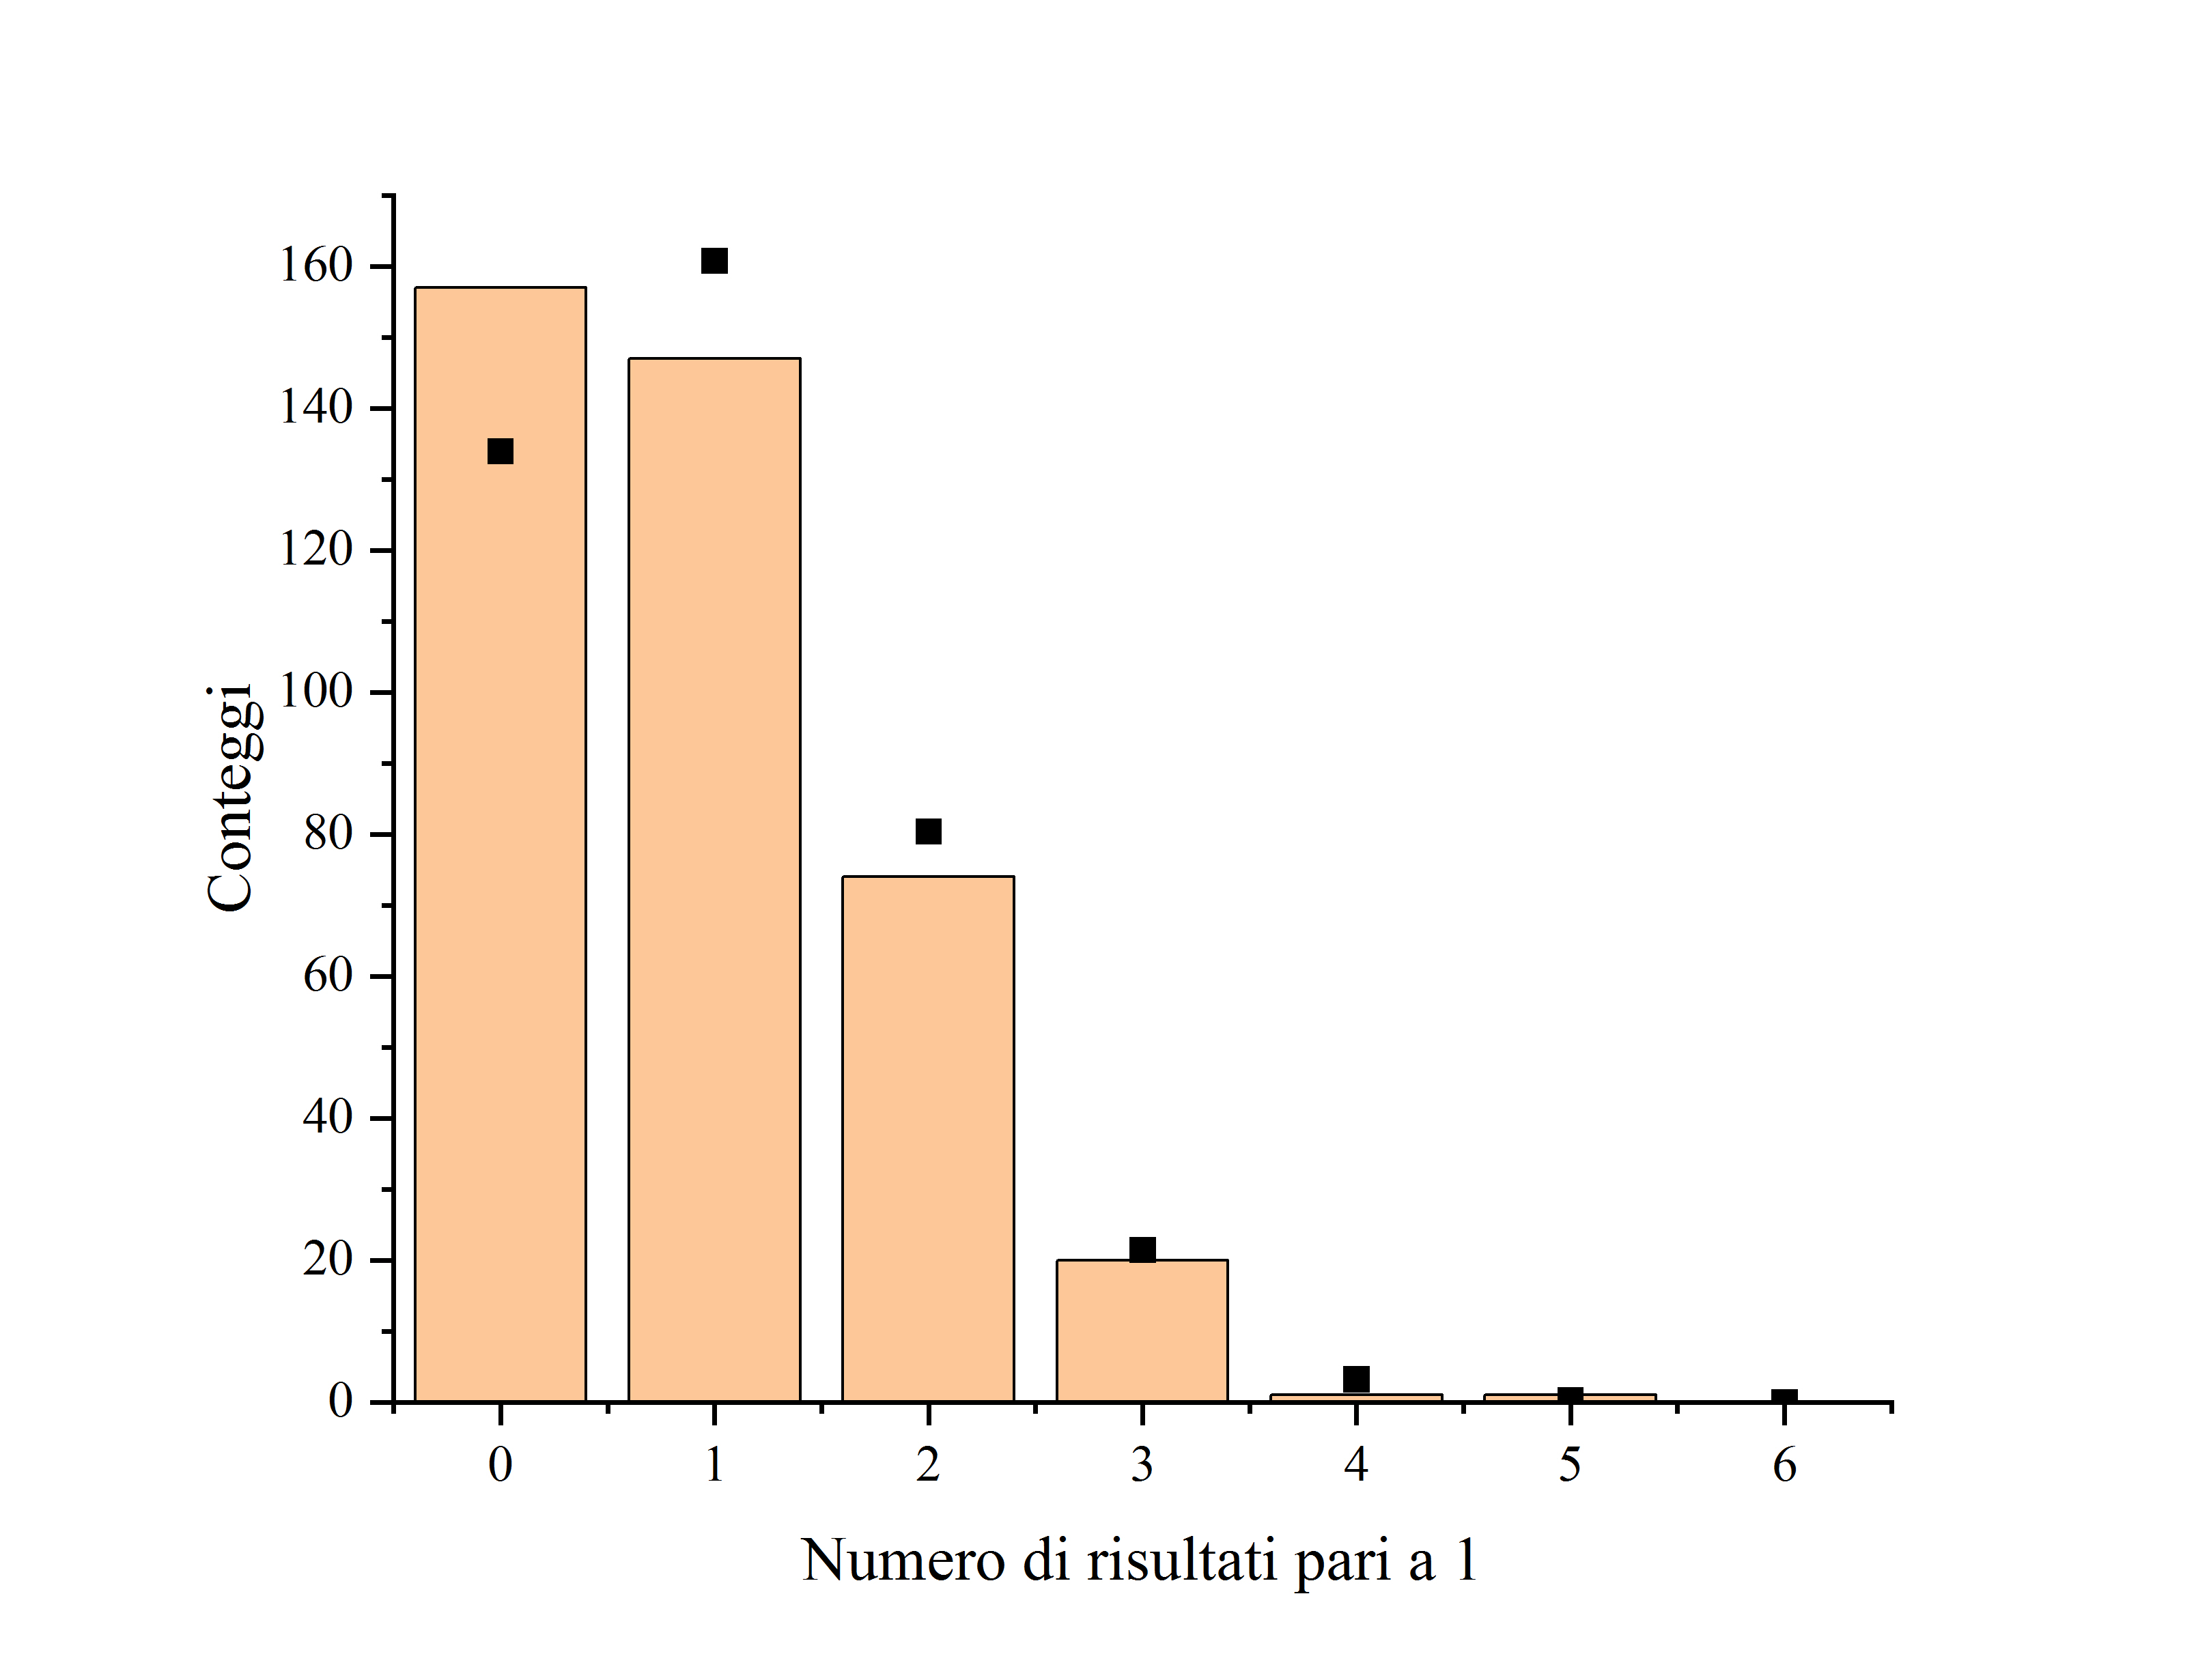
\includegraphics[trim={2cm .5cm 2.4cm 2.1cm},clip,width=.5\textwidth]{img/Dadi1.jpg}
        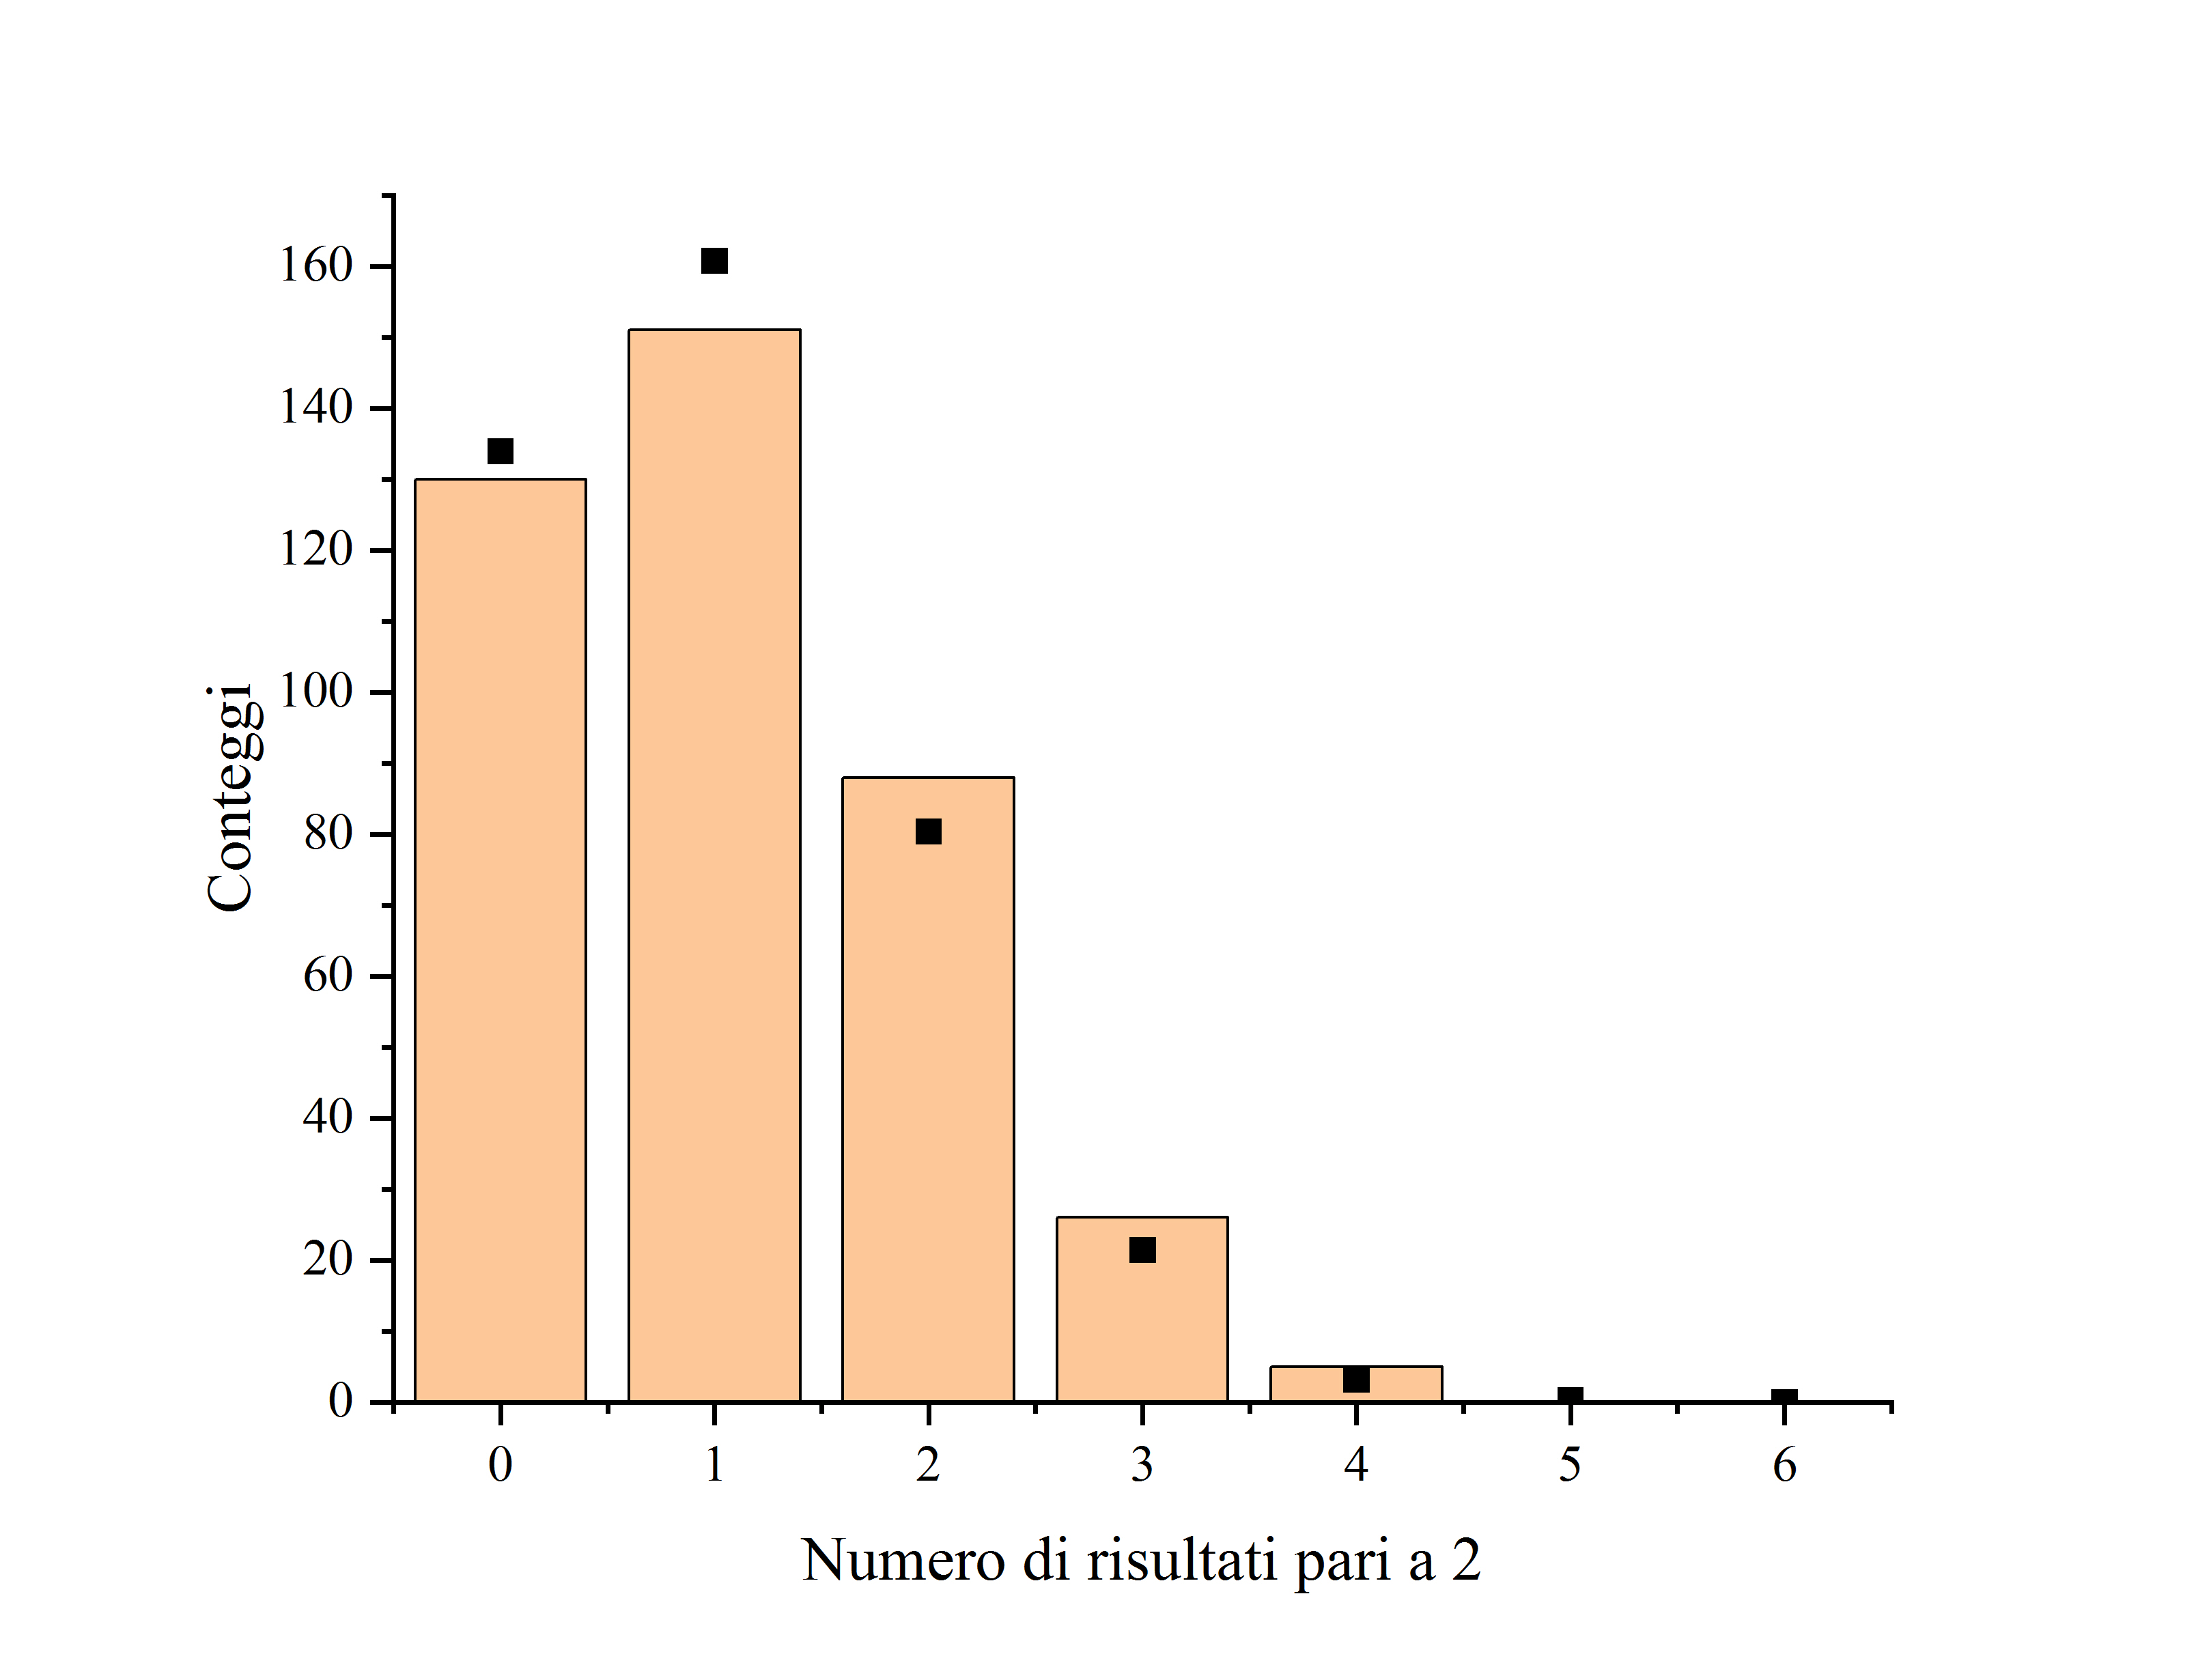
\includegraphics[trim={2cm .5cm 2.4cm 2.1cm},clip,width=.5\textwidth]{img/Dadi2.jpg}
        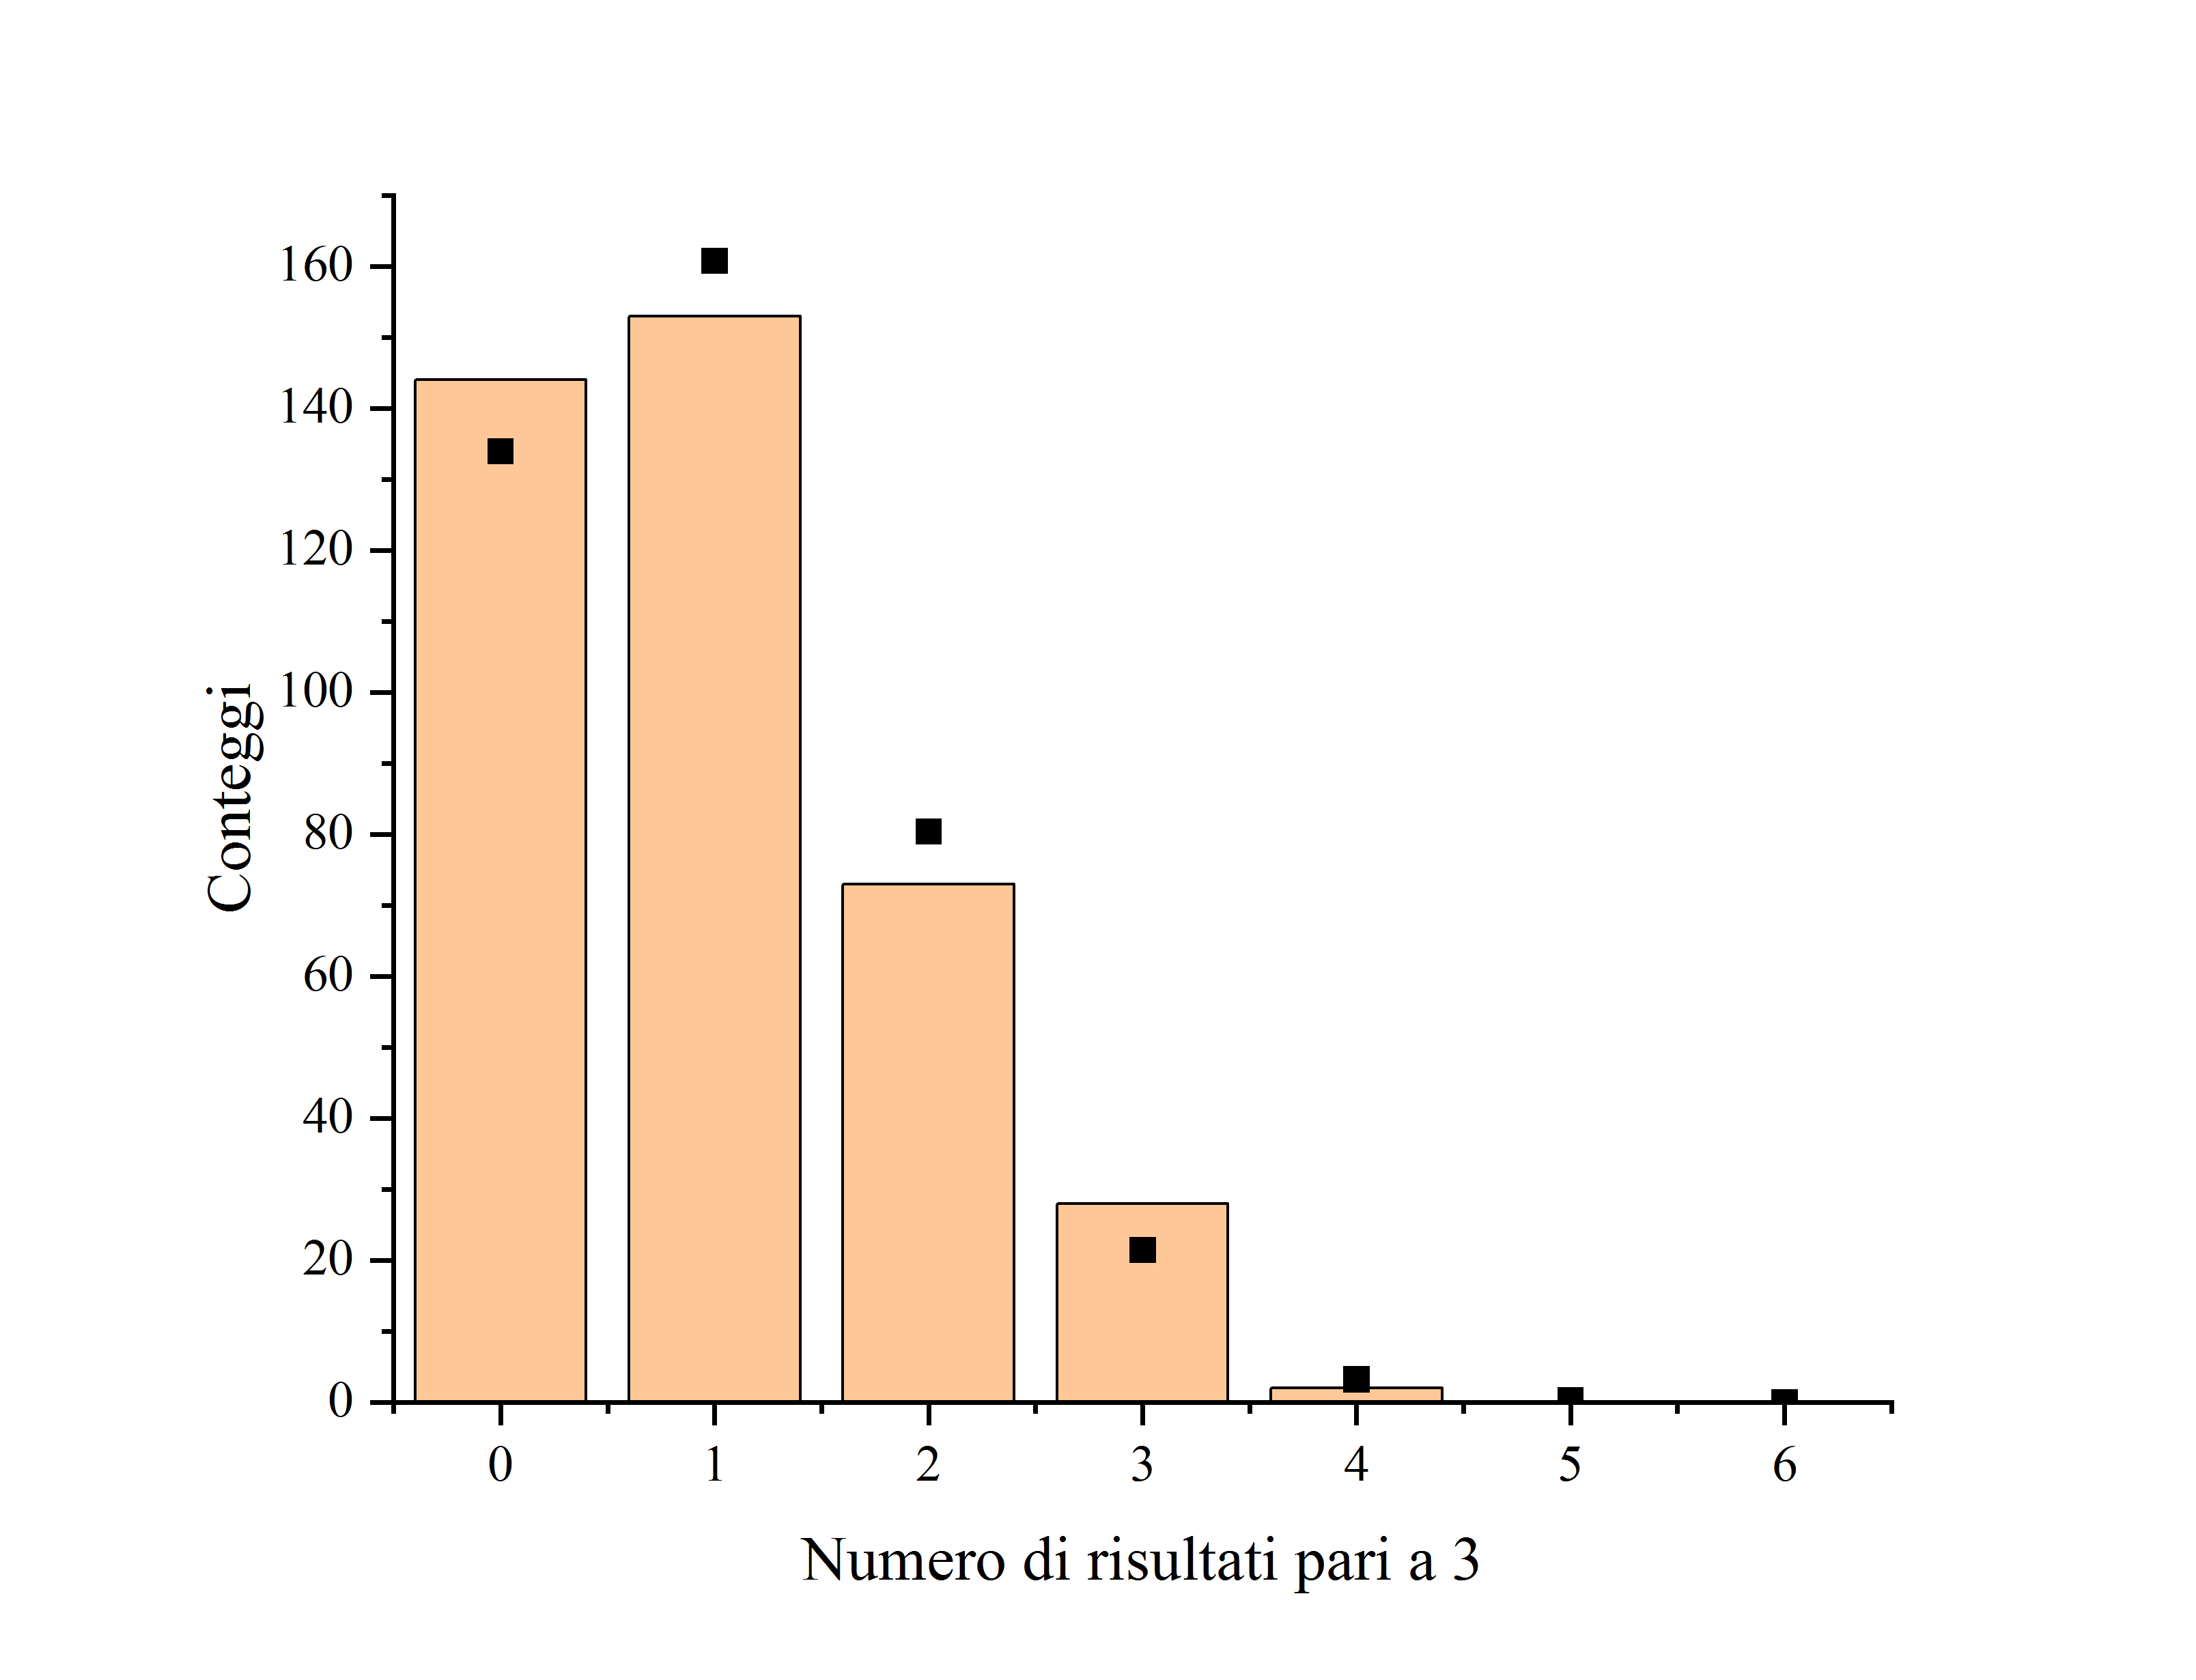
\includegraphics[trim={2cm .5cm 2.4cm 2.1cm},clip,width=.5\textwidth]{img/Dadi3.jpg}
        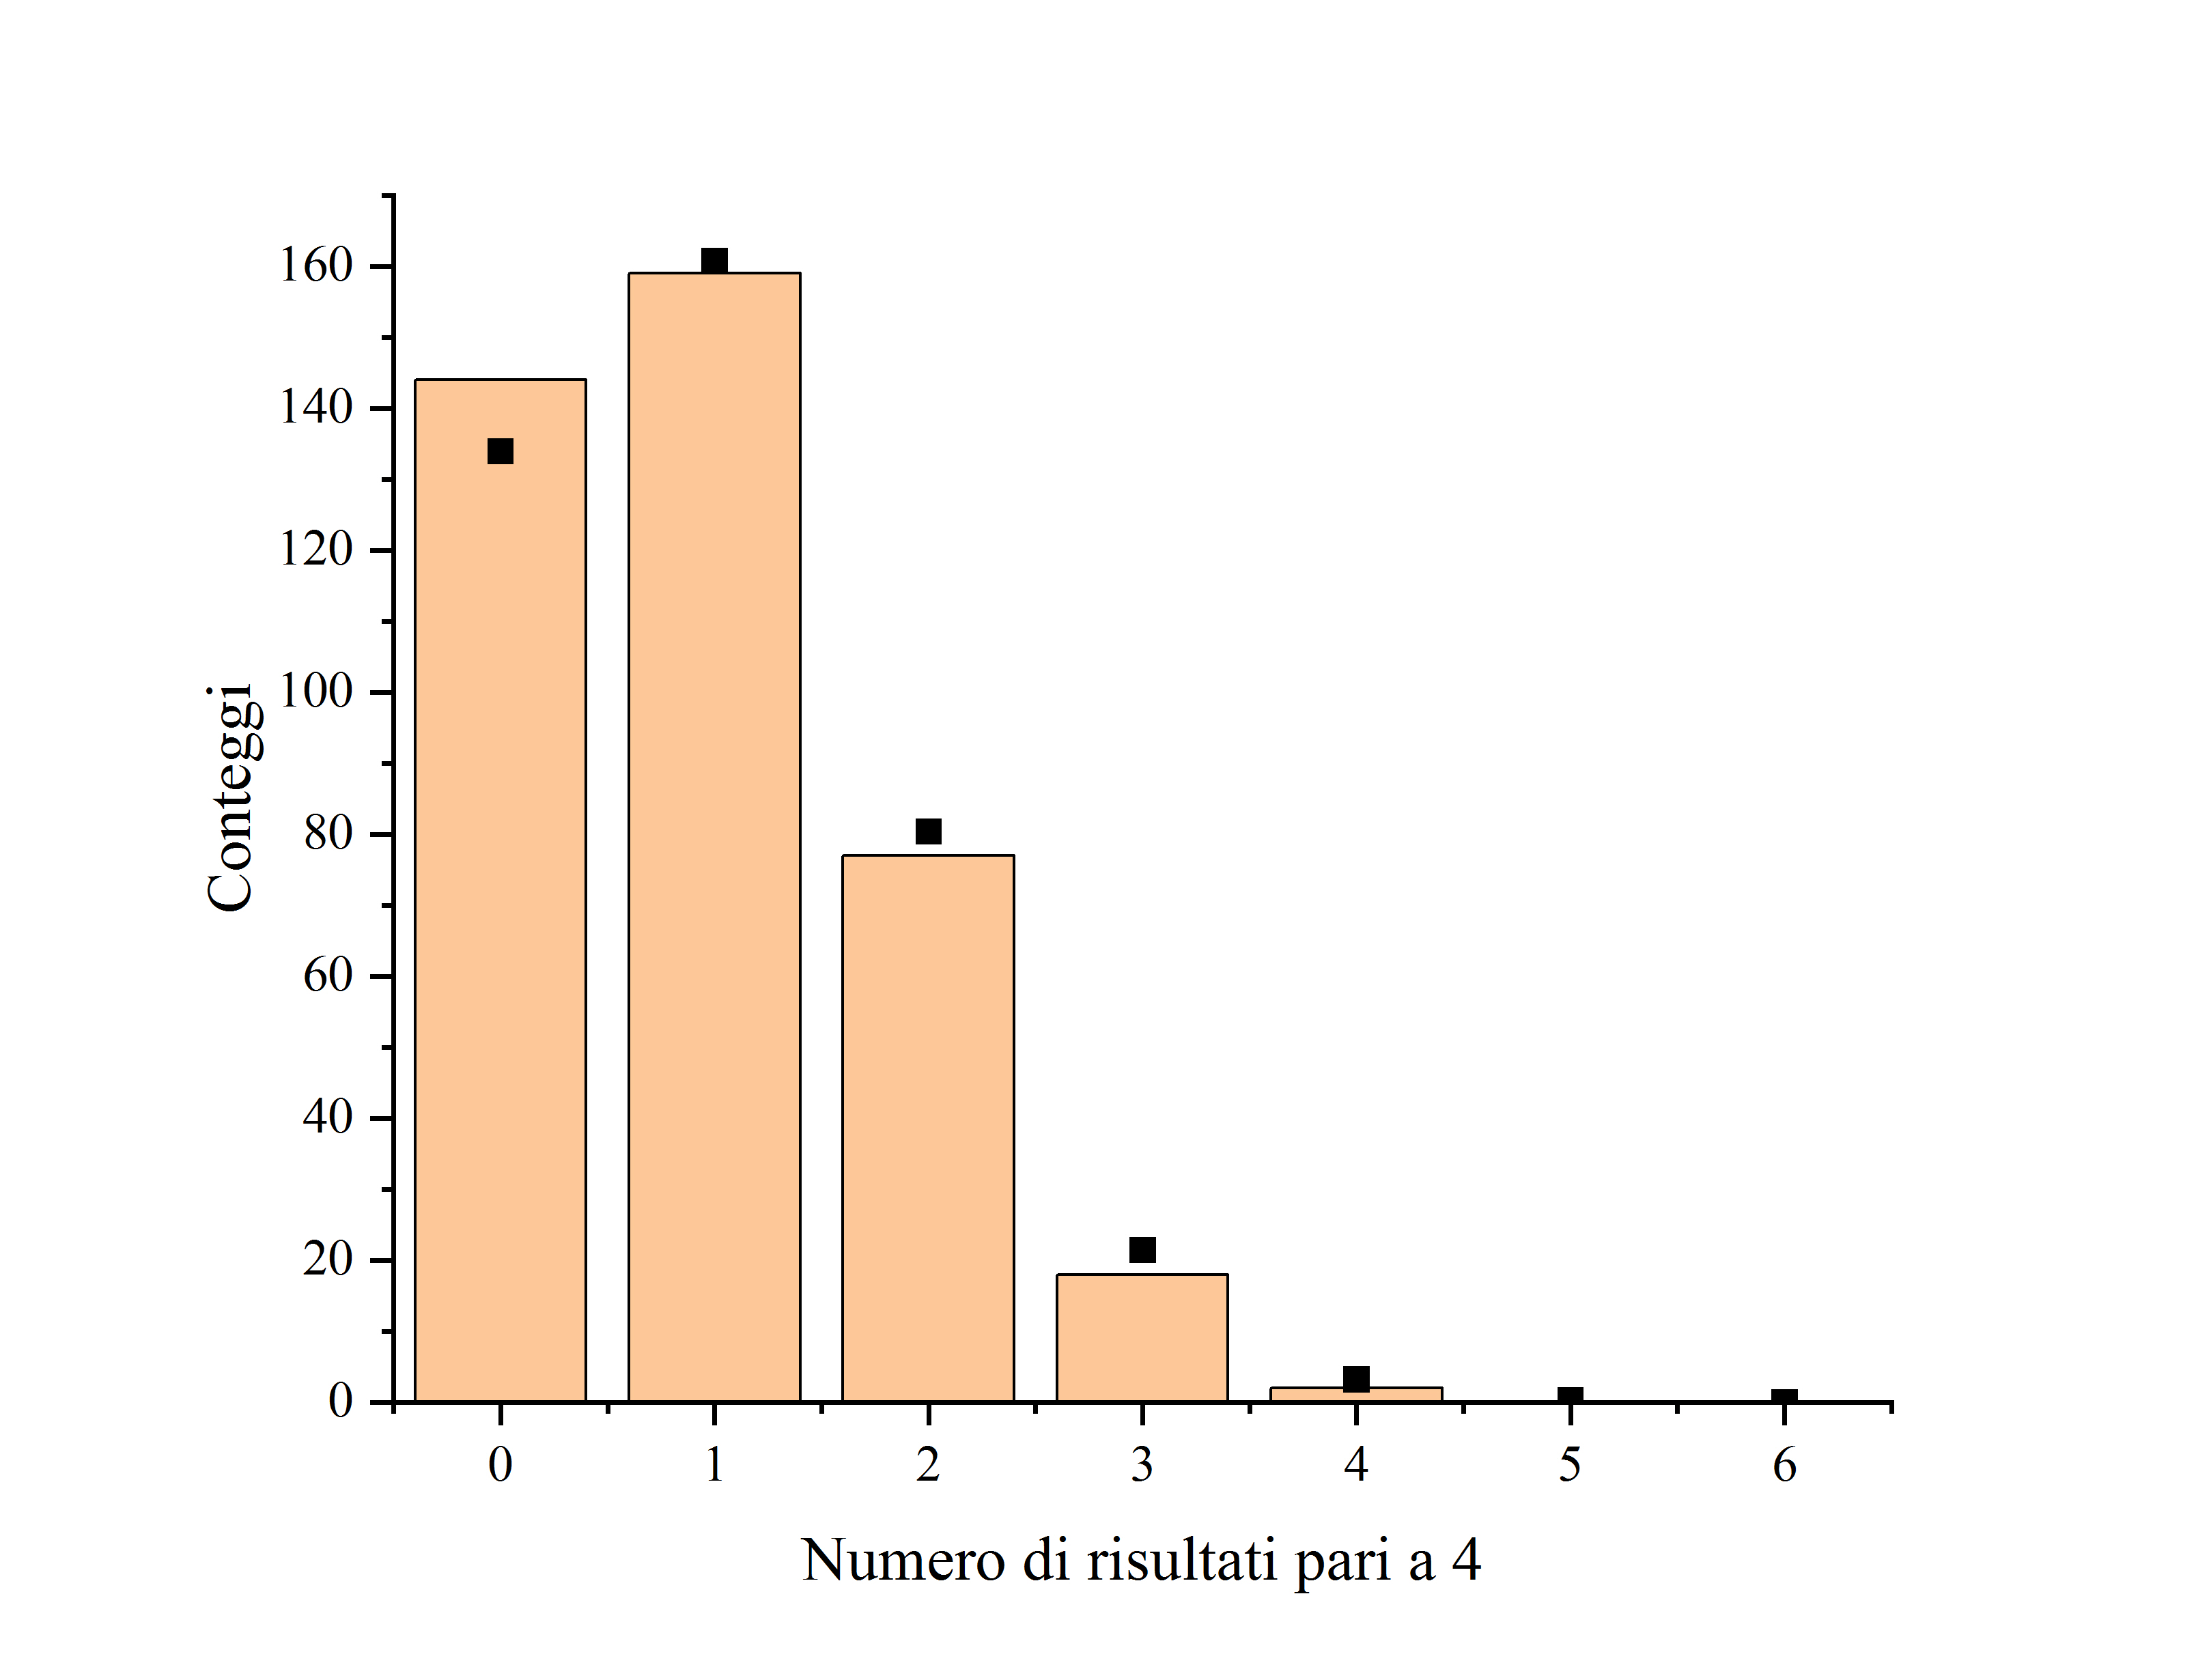
\includegraphics[trim={2cm .5cm 2.4cm 2.1cm},clip,width=.5\textwidth]{img/Dadi4.jpg}
        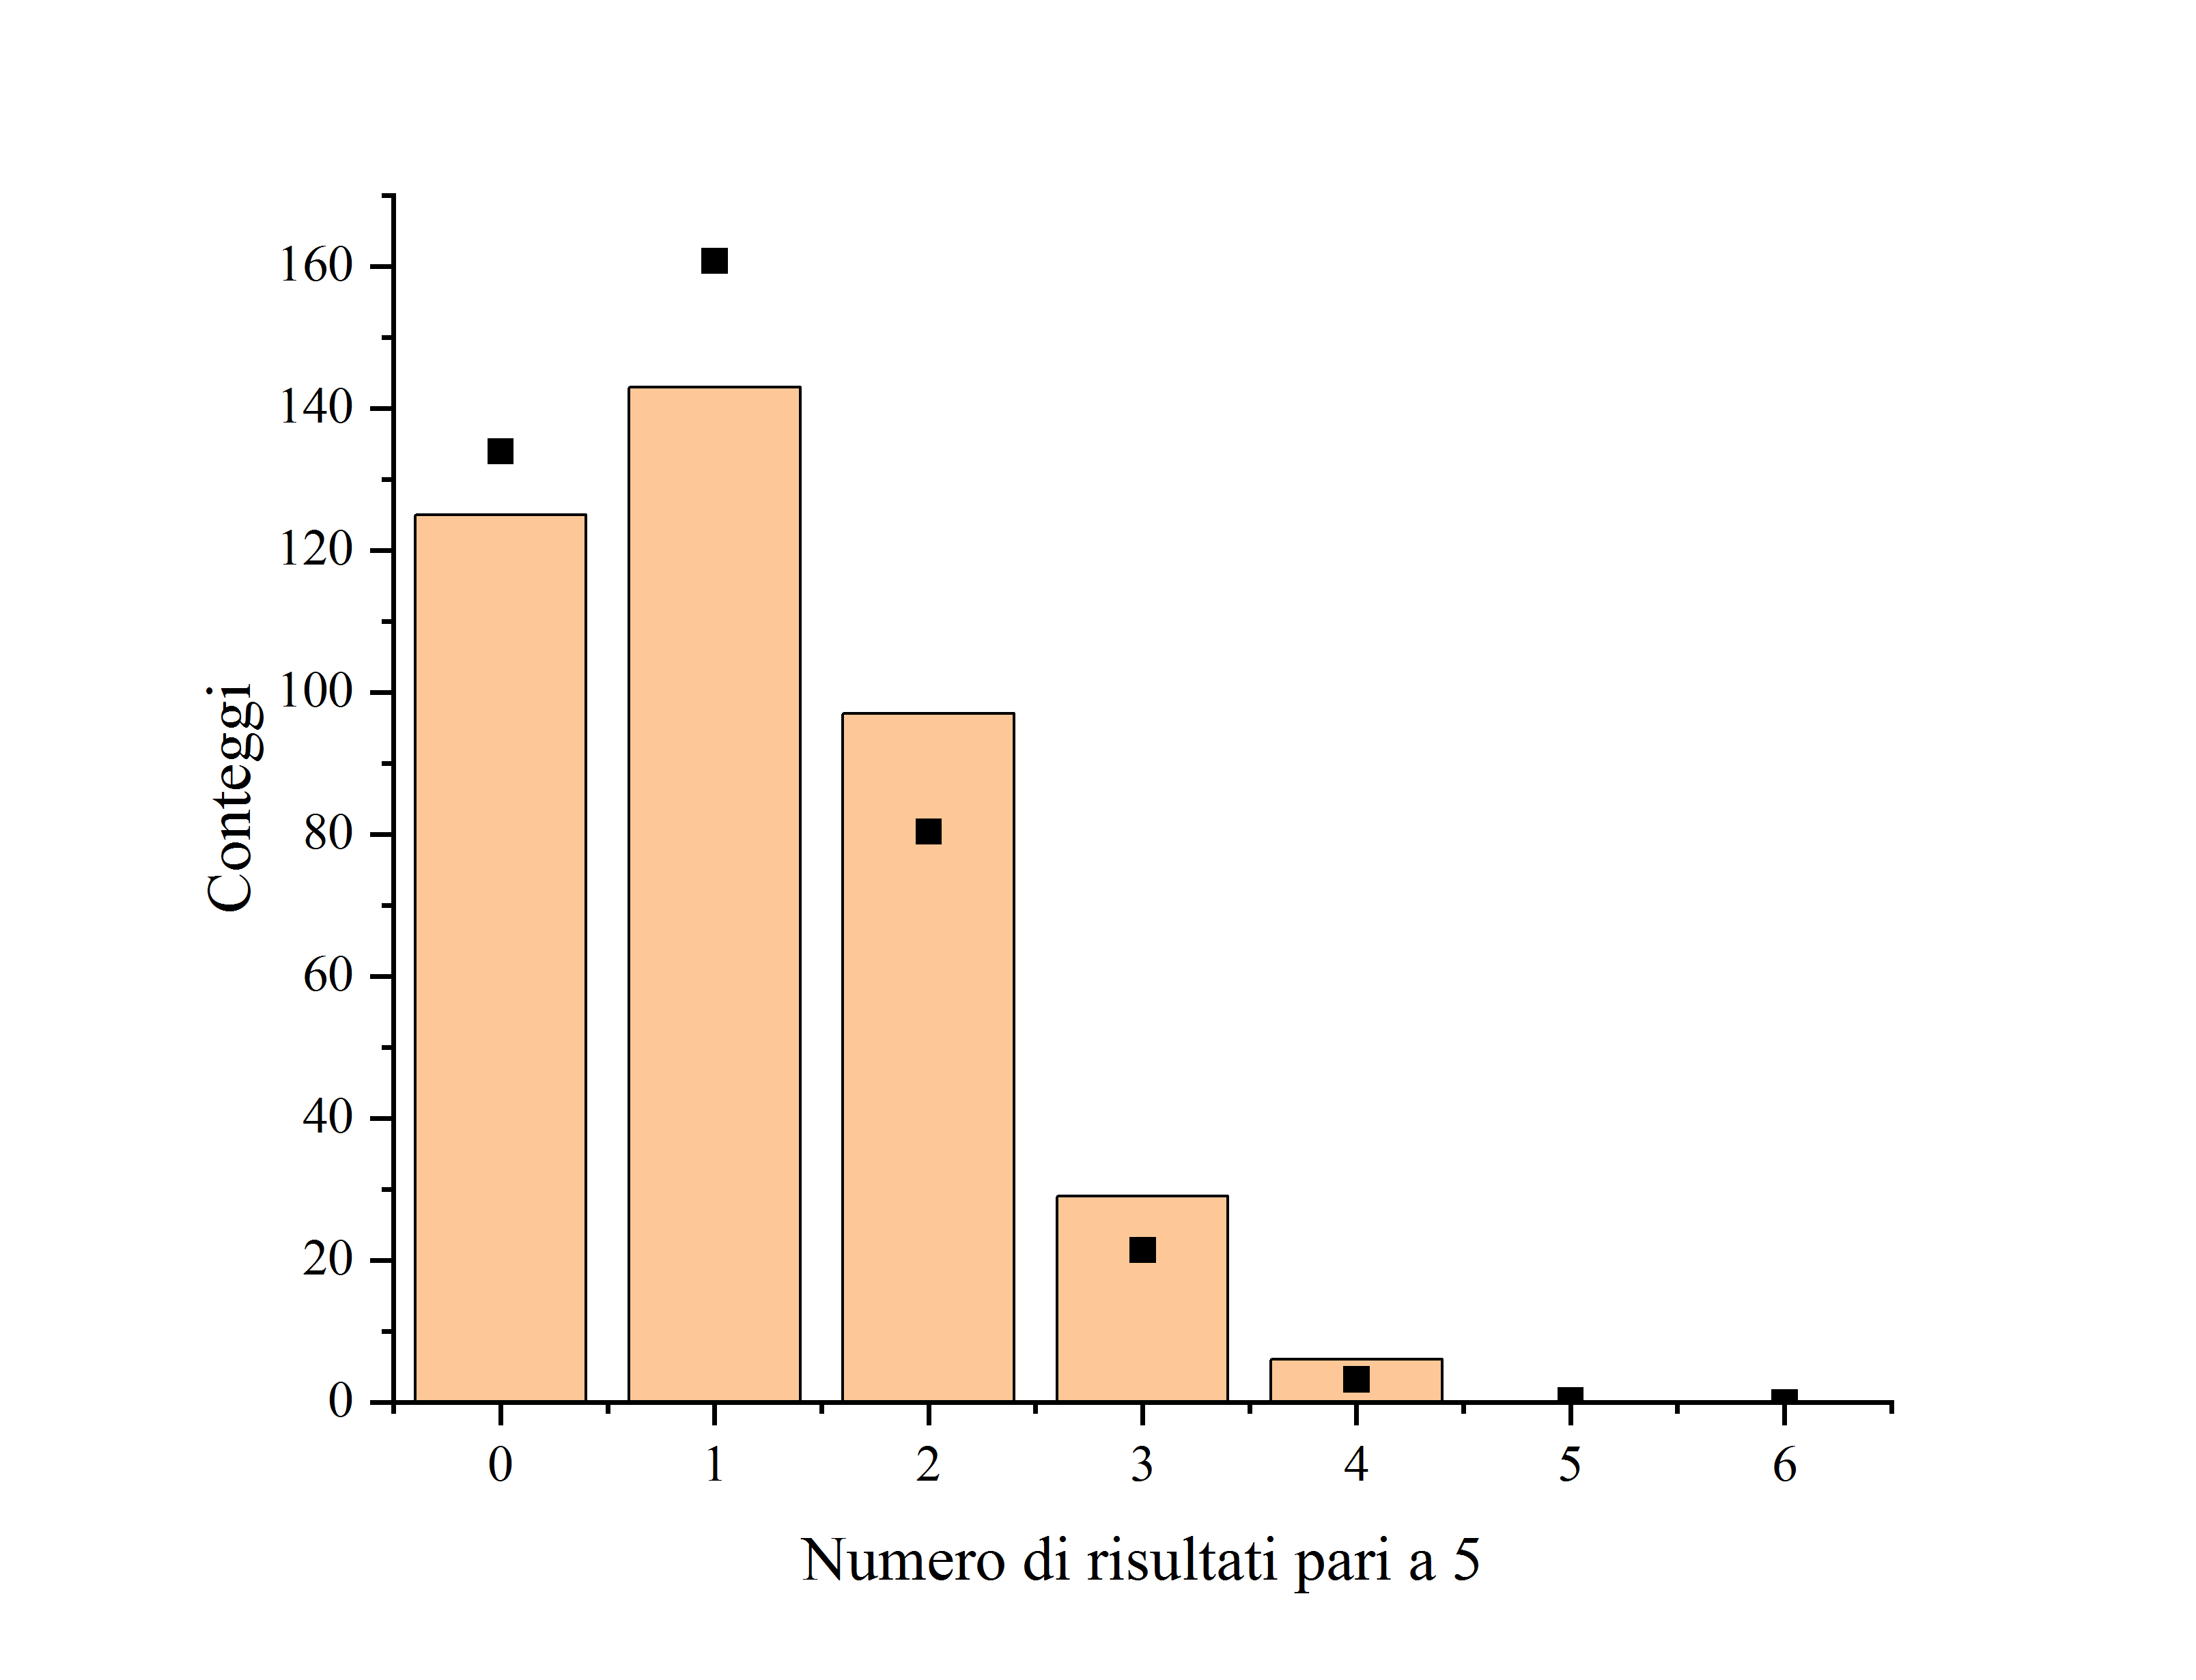
\includegraphics[trim={2cm .5cm 2.4cm 2.1cm},clip,width=.5\textwidth]{img/Dadi5.jpg}
        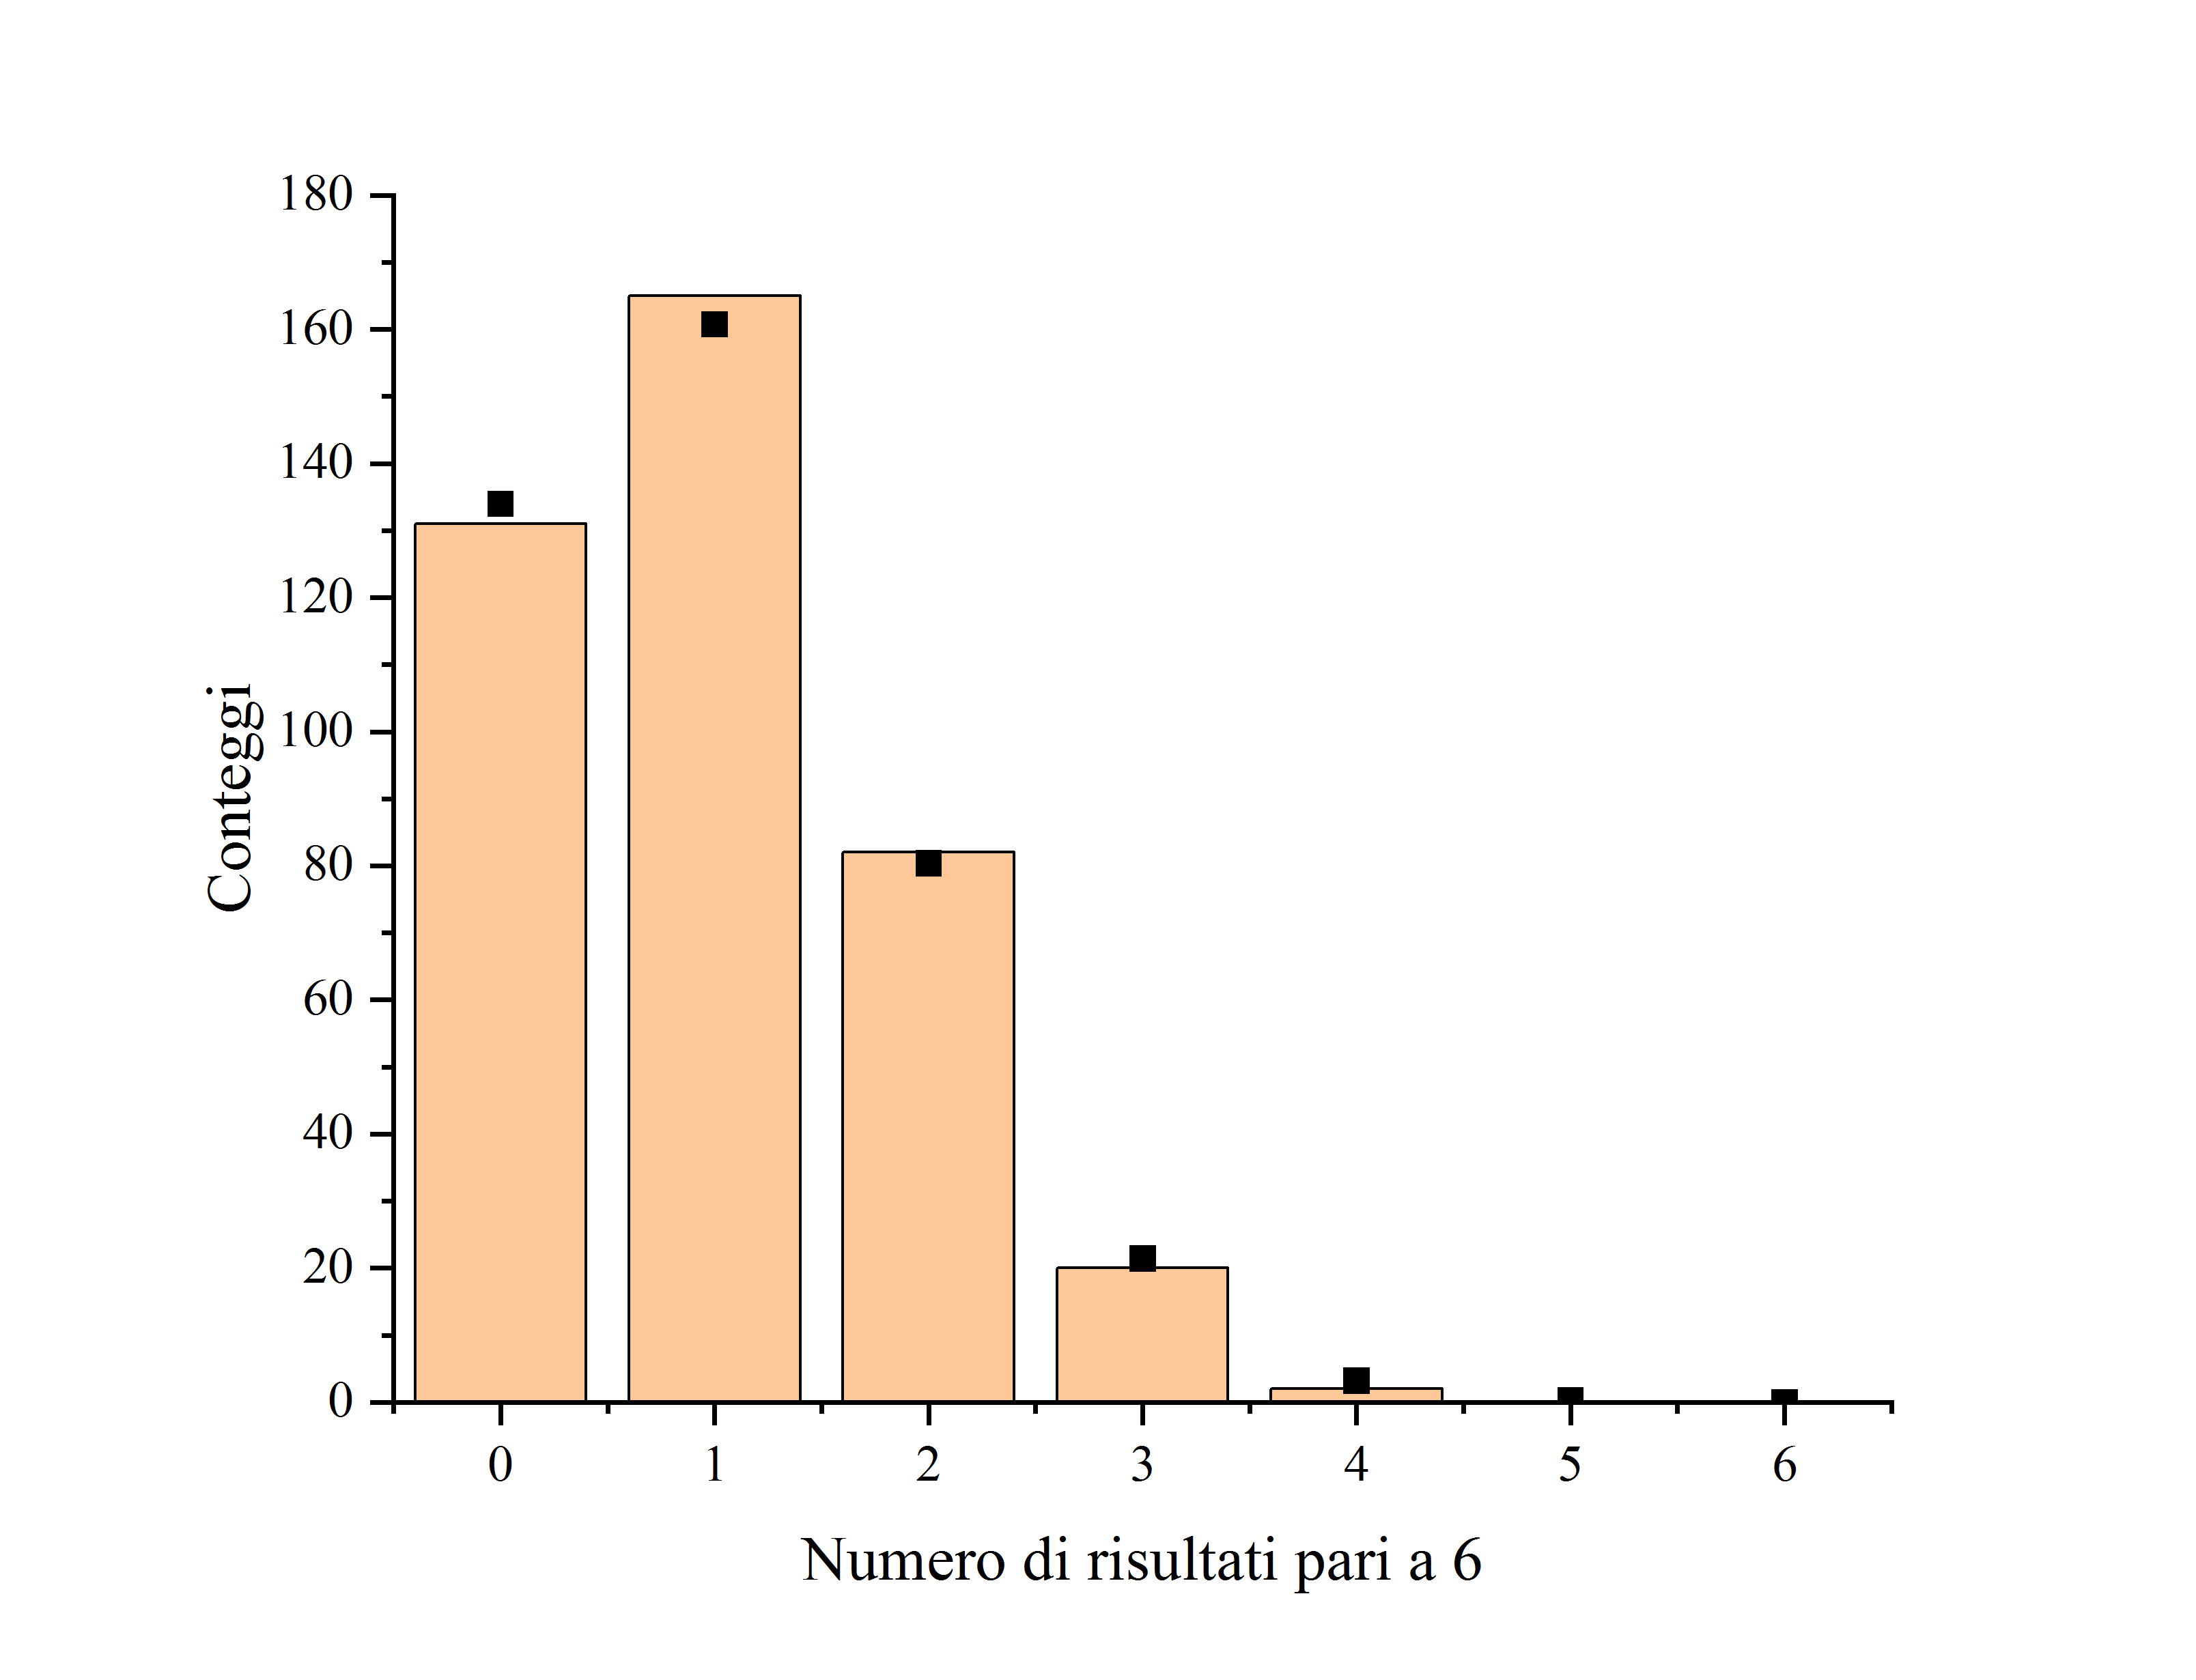
\includegraphics[trim={2cm .5cm 2.4cm 2.1cm},clip,width=.5\textwidth]{img/Dadi6.jpg}
    \end{figure}
\end{center}

Come è possibile osservare da questi grafici, i risultati riportati sembrano seguire
grossomodo la distribuzione teorica. Tuttavia, presentano deviazioni osservabili; il
gruppo di lavoro ritiene che ciò sia principalmente dovuto al ridotto numero di lanci.

% \subsubsection*{Onestà dei dadi}
% Avendo segnato tutti i risultati di ogni dado, possiamo inoltre stimare se i dadi che
% abbiamo utilizzato sono truccati o meno. Infatti, su un dado onesto ci aspettiamo
% che escano tutti i risultati possibili con equa probabilità. Di seguito riportiamo
% gli istogrammi dei valori usciti su ogni dado.

% \begin{figure*}
%     \caption{...}
% \end{figure*}

\subsection{Simulazione}
Tramite un programma da noi scritto e compilato\footnote{\emph{Vedi} Appendice A},
simuliamo la stessa esperienza con $10^{12}$ lanci dei sei dadi, al fine di
verificare la legge dei grandi numeri.

Di seguito riportiamo, in un istogramma, i risultati della simulazione.

\begin{center}
    \begin{figure}[H]
        % trim={< v > ^}
        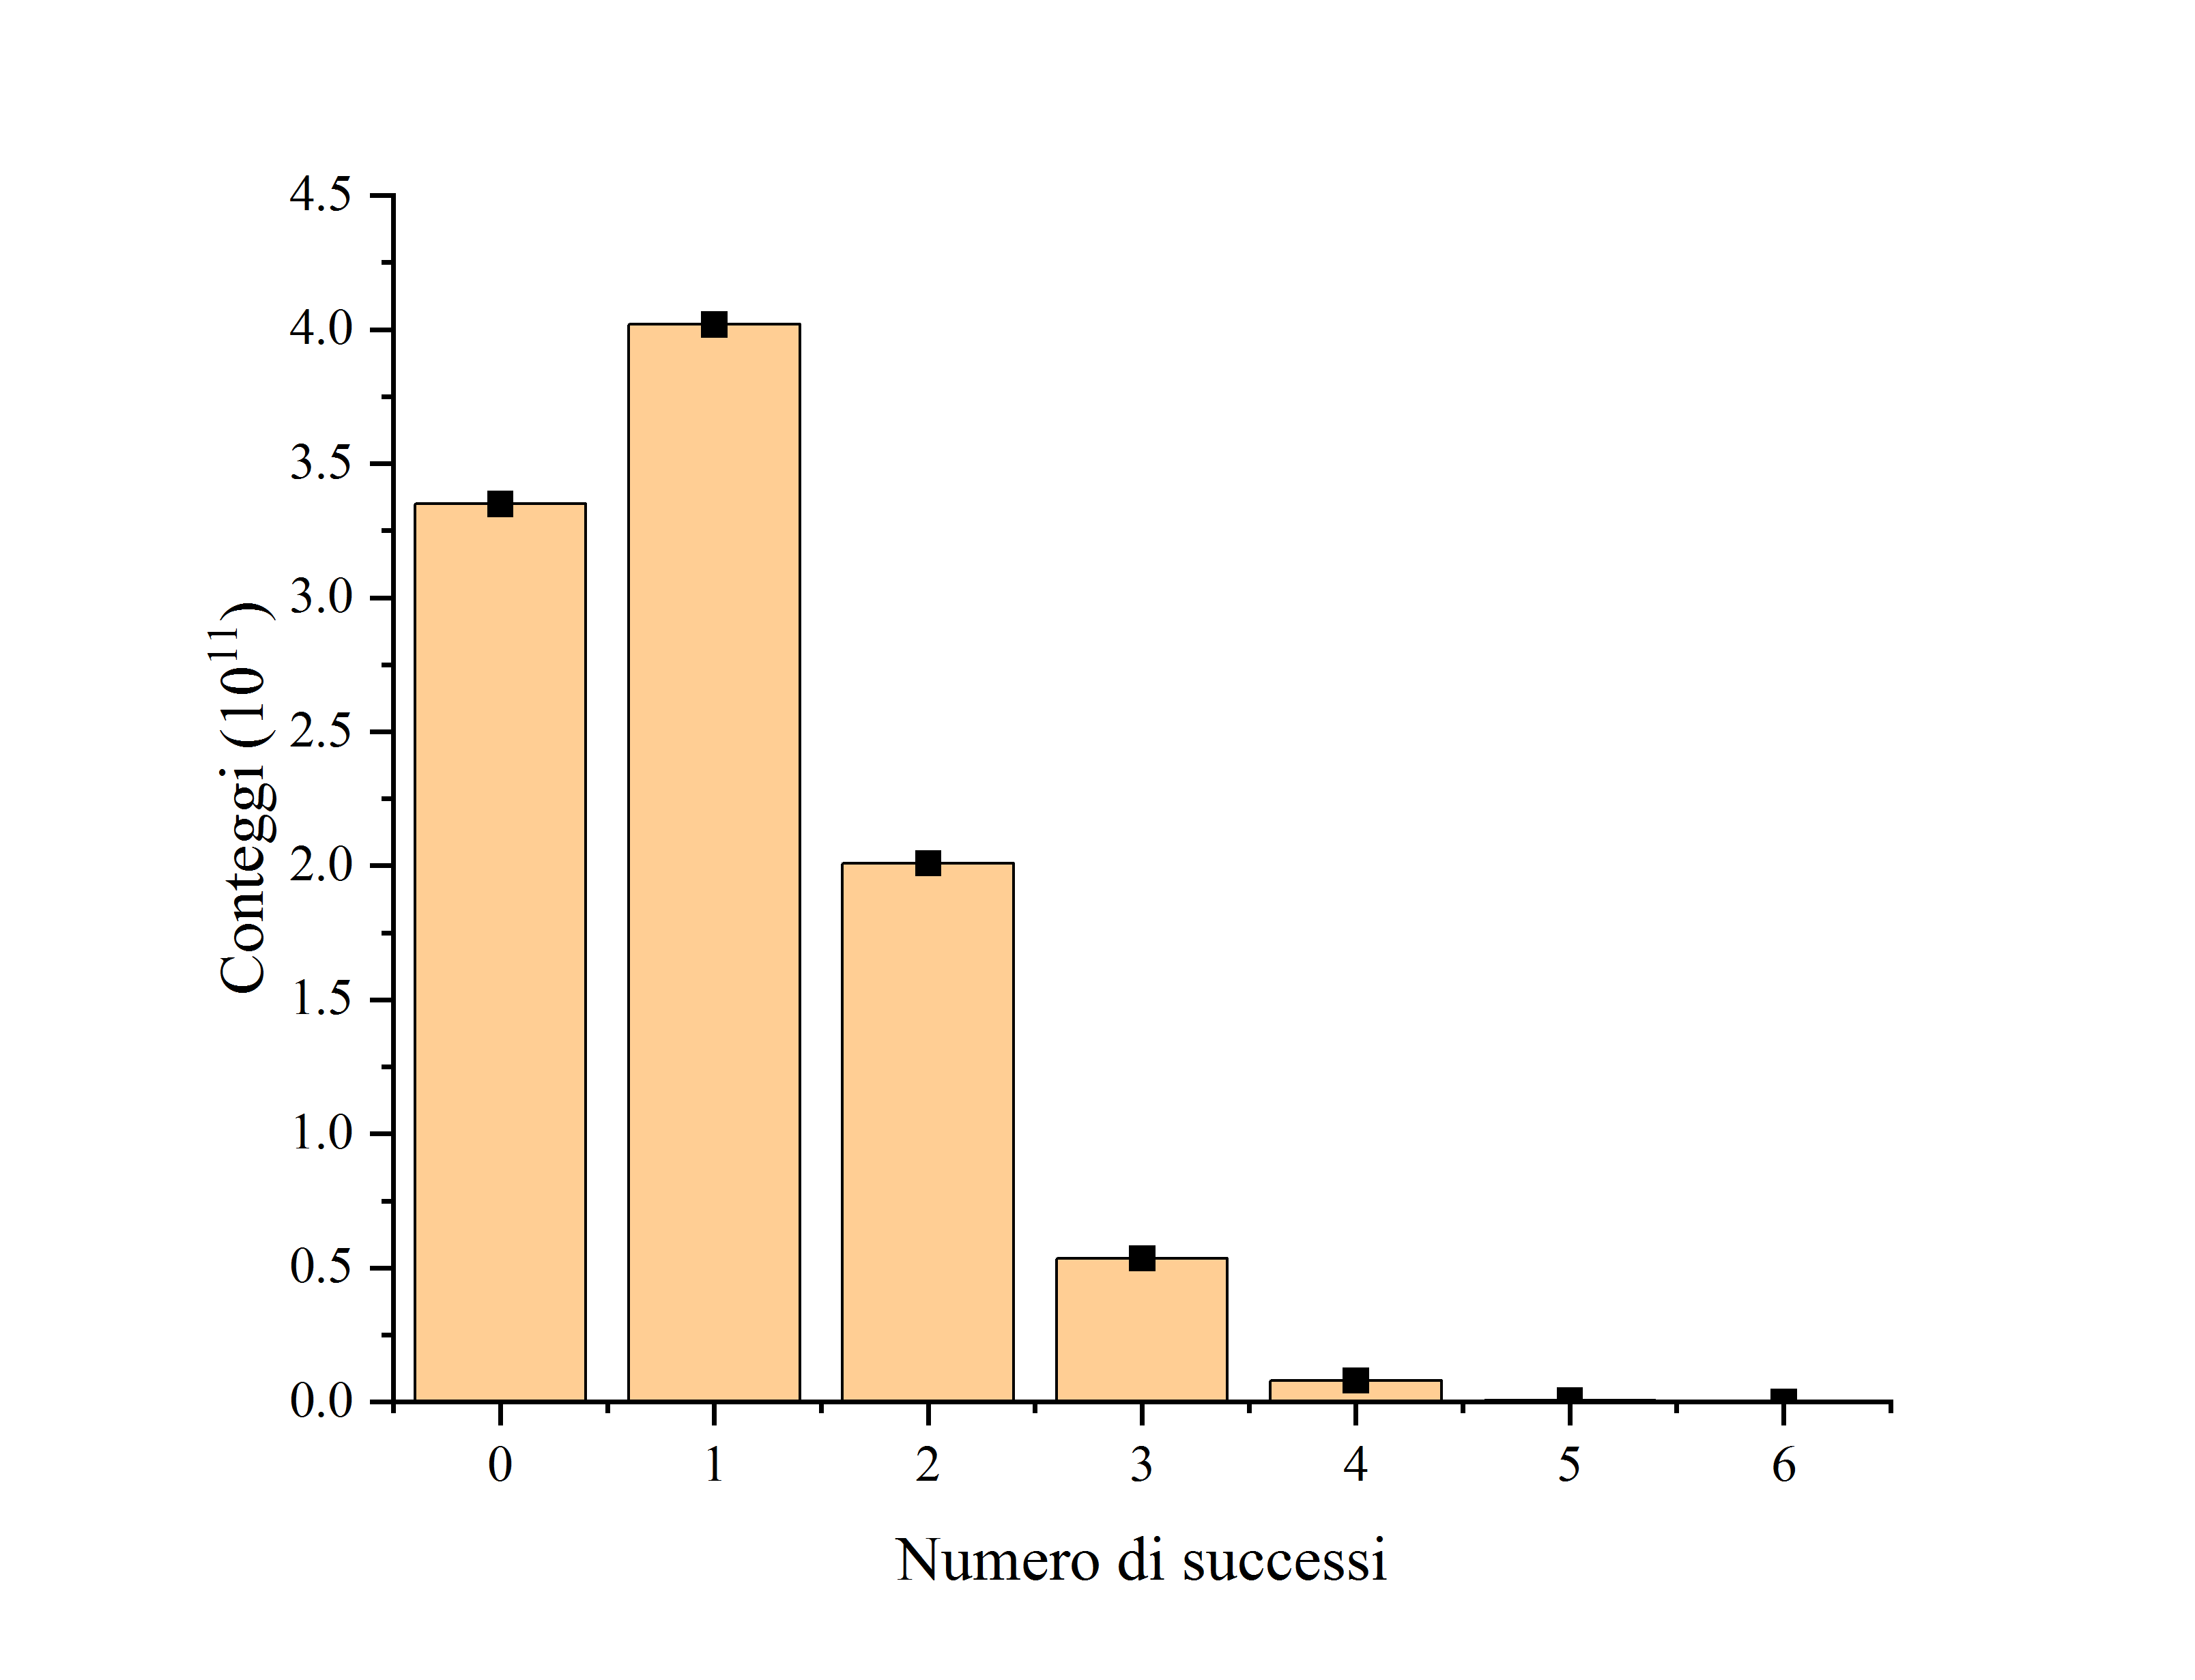
\includegraphics[trim={2cm .5cm 2cm 2.1cm},clip,width=\textwidth]{img/DadiSimul.png}
    \end{figure}
\end{center}

Come è possibile osservare dal grafico, i risultati della simulazione sono, in proporzione,
talmente vicini alla distribuzione teorica da risultare pressoché indistinguibili.

Ciò è in accordo con la legge dei grandi numeri, secondo la quale, al crescere del
numero di prove, la distribuzione di probabilità rappresenta sempre meglio i
risultati ottenuti, normalizzati.

\pagebreak
\section{Processo di Poisson}
\subsection{Materiali e strumenti di misura utilizzati}
\begin{center}
    \begin{tblr}{ |Q[l,m]|Q[c,m]|Q[c,m]|Q[c,m]| }
        \hline
        \textbf{Strumento di misura} & \textbf{\:\:\:\:\:Soglia\:\:\:\:\:} & \textbf{Portata} & \textbf{Sensibilità} \\
        \hline
        {Contatore Geiger} & \qty{1}{conteggi \per s} & N./A. & \qty{1}{conteggi \per s} \\
        \hline[dashed]
        Metro a nastro & \qty{0.1}{cm} & \qty{300.0}{cm} & \qty{0.1}{cm} \\
        \hline
        \hline
        \textbf{Altro} & \SetCell[c=3]{l} \textbf{Descrizione/Note} \\
        \hline
        {Campione di $\Th$} & \SetCell[c=3]{l} {
            Componente di una lampada da campeggio
        } \\
        \hline
    \end{tblr}
\end{center}


\subsection{Esperienza e procedimento di misura}

Posizionato il contatore Geiger a una certa distanza $d_i$ dal campione di $\Th$
(con $i\in\left[1;4\right]\cap\mathbb{N}$),
definiamo una variabile aleatoria $x_\gamma$ come il numero di raggi $\gamma$
emessi dal $\Th$ nell'arco di un secondo, nella direzione del contatore.
Allora, detta $\overline{x_\gamma}$ la media teorica
% \footnote{
    % Che il parametro della distribuzione coincida con la media è facilmente
    % dimostrabile. Detto $\lambda$ quel parametro, vale:
    % \[\begin{aligned}
        % \overline{x_\gamma} &= \sum_{k=0}^{+\infty} k\,p(x_\gamma=k) =
        % \sum_{k=0}^{+\infty} k \frac{\lambda^k  e^{-\lambda}}{k!} =
        % e^{-\lambda} \sum_{k=0}^{+\infty} k \frac{\lambda^k}{k!} =
        % e^{-\lambda} \left(0 + \sum_{k=1}^{+\infty} k \frac{\lambda^k}{k!}\right) \\ &=
        % \lambda e^{-\lambda} \sum_{k=1}^{+\infty} \frac{\lambda^{k-1}}{(k-1)!} =
        % \lambda e^{-\lambda} \sum_{j=0}^{+\infty} \frac{\lambda^j}{j!} =
        % \lambda e^{-\lambda} e^\lambda =
        % \lambda\quad\square
    % \end{aligned}\]
% }
di $x_\gamma$, la distribuzione di probabilità di $x_\gamma$ è data da una Poissoniana:
\[
    p(x_\gamma=k)=\frac{\overline{x_\gamma}^k e^{-\overline{x_\gamma}}}{k!}
    \qquad
    \forall k\in\mathbb{N}
\]
Il valore di $\overline{x_\gamma}$ è legato alla distanza $d_i$ e al tempo
di dimezzamento del $\Th$ ($T_{1/2}$) secondo la seguente relazione:
% TODO
% \footnote{
%     Dimostrazione:
%     \[*\]
% }
\[\overline{x_\gamma} = \frac{r^2\ln{2}}{4 T_{1/2}}N d_i^{-2} + \gamma_0\]

Per un tempo complessivo di circa un'ora\footnote{
    Abbiamo scelto deliberatamente di acquisire esattamente 3657 secondi in quanto
    $3657$ minimizza la funzione
    $f(x)=\left\{\frac{x}{\pi}\right\}=\frac{x}{\pi} - \left\lfloor\frac{x}{\pi}\right\rfloor$
    meglio di $3600$.
} ($\qty{3657}{s}$).

Infine, il gruppo di lavoro ha acquisito, sempre per $\qty{3657}{s}$,
i conteggi al secondo di raggi $\gamma$ nella direzione opposta rispetto
al campione, per avere una stima della radioattività ambientale.

\emph{
    \textbf{Notazione.} Indichiamo con $\gamma_i$ complessivamente i conteggi
    acquisiti a distanza $d_i$ dal campione
    (con $i\in\left[1;4\right]\cap\mathbb{N}$).
    Allora $\overline{\gamma_i}$ sarà la media della distribuzione, dove
    $\bestp{\overline{\gamma_i}}$ sarà la media dei conteggi,
    mentre $\sigma_{\gamma_i}$ sarà la deviazione standard e
    $
        \delta\!\left(\overline{\gamma_i}\right) =
        \sigma_{\overline{\gamma_i}} =
        \frac{\sigma_{\gamma_i}}{\sqrt{3657}}
    $
    l'errore sulla media.
    Analogamente per \emph{
        $\gamma_\text{amb}$,
        $\gamma_\text{amb}$ e
        $\overline{\gamma_\text{amb}}$.
    }
}

Di seguito, riportiamo, come istogrammi, le distribuzioni di tutti i $\gamma_i$,
a cui abbiamo sovrapposto i valori attesi

\begin{center}
    \begin{figure}[H]
        % trim={< v > ^}
        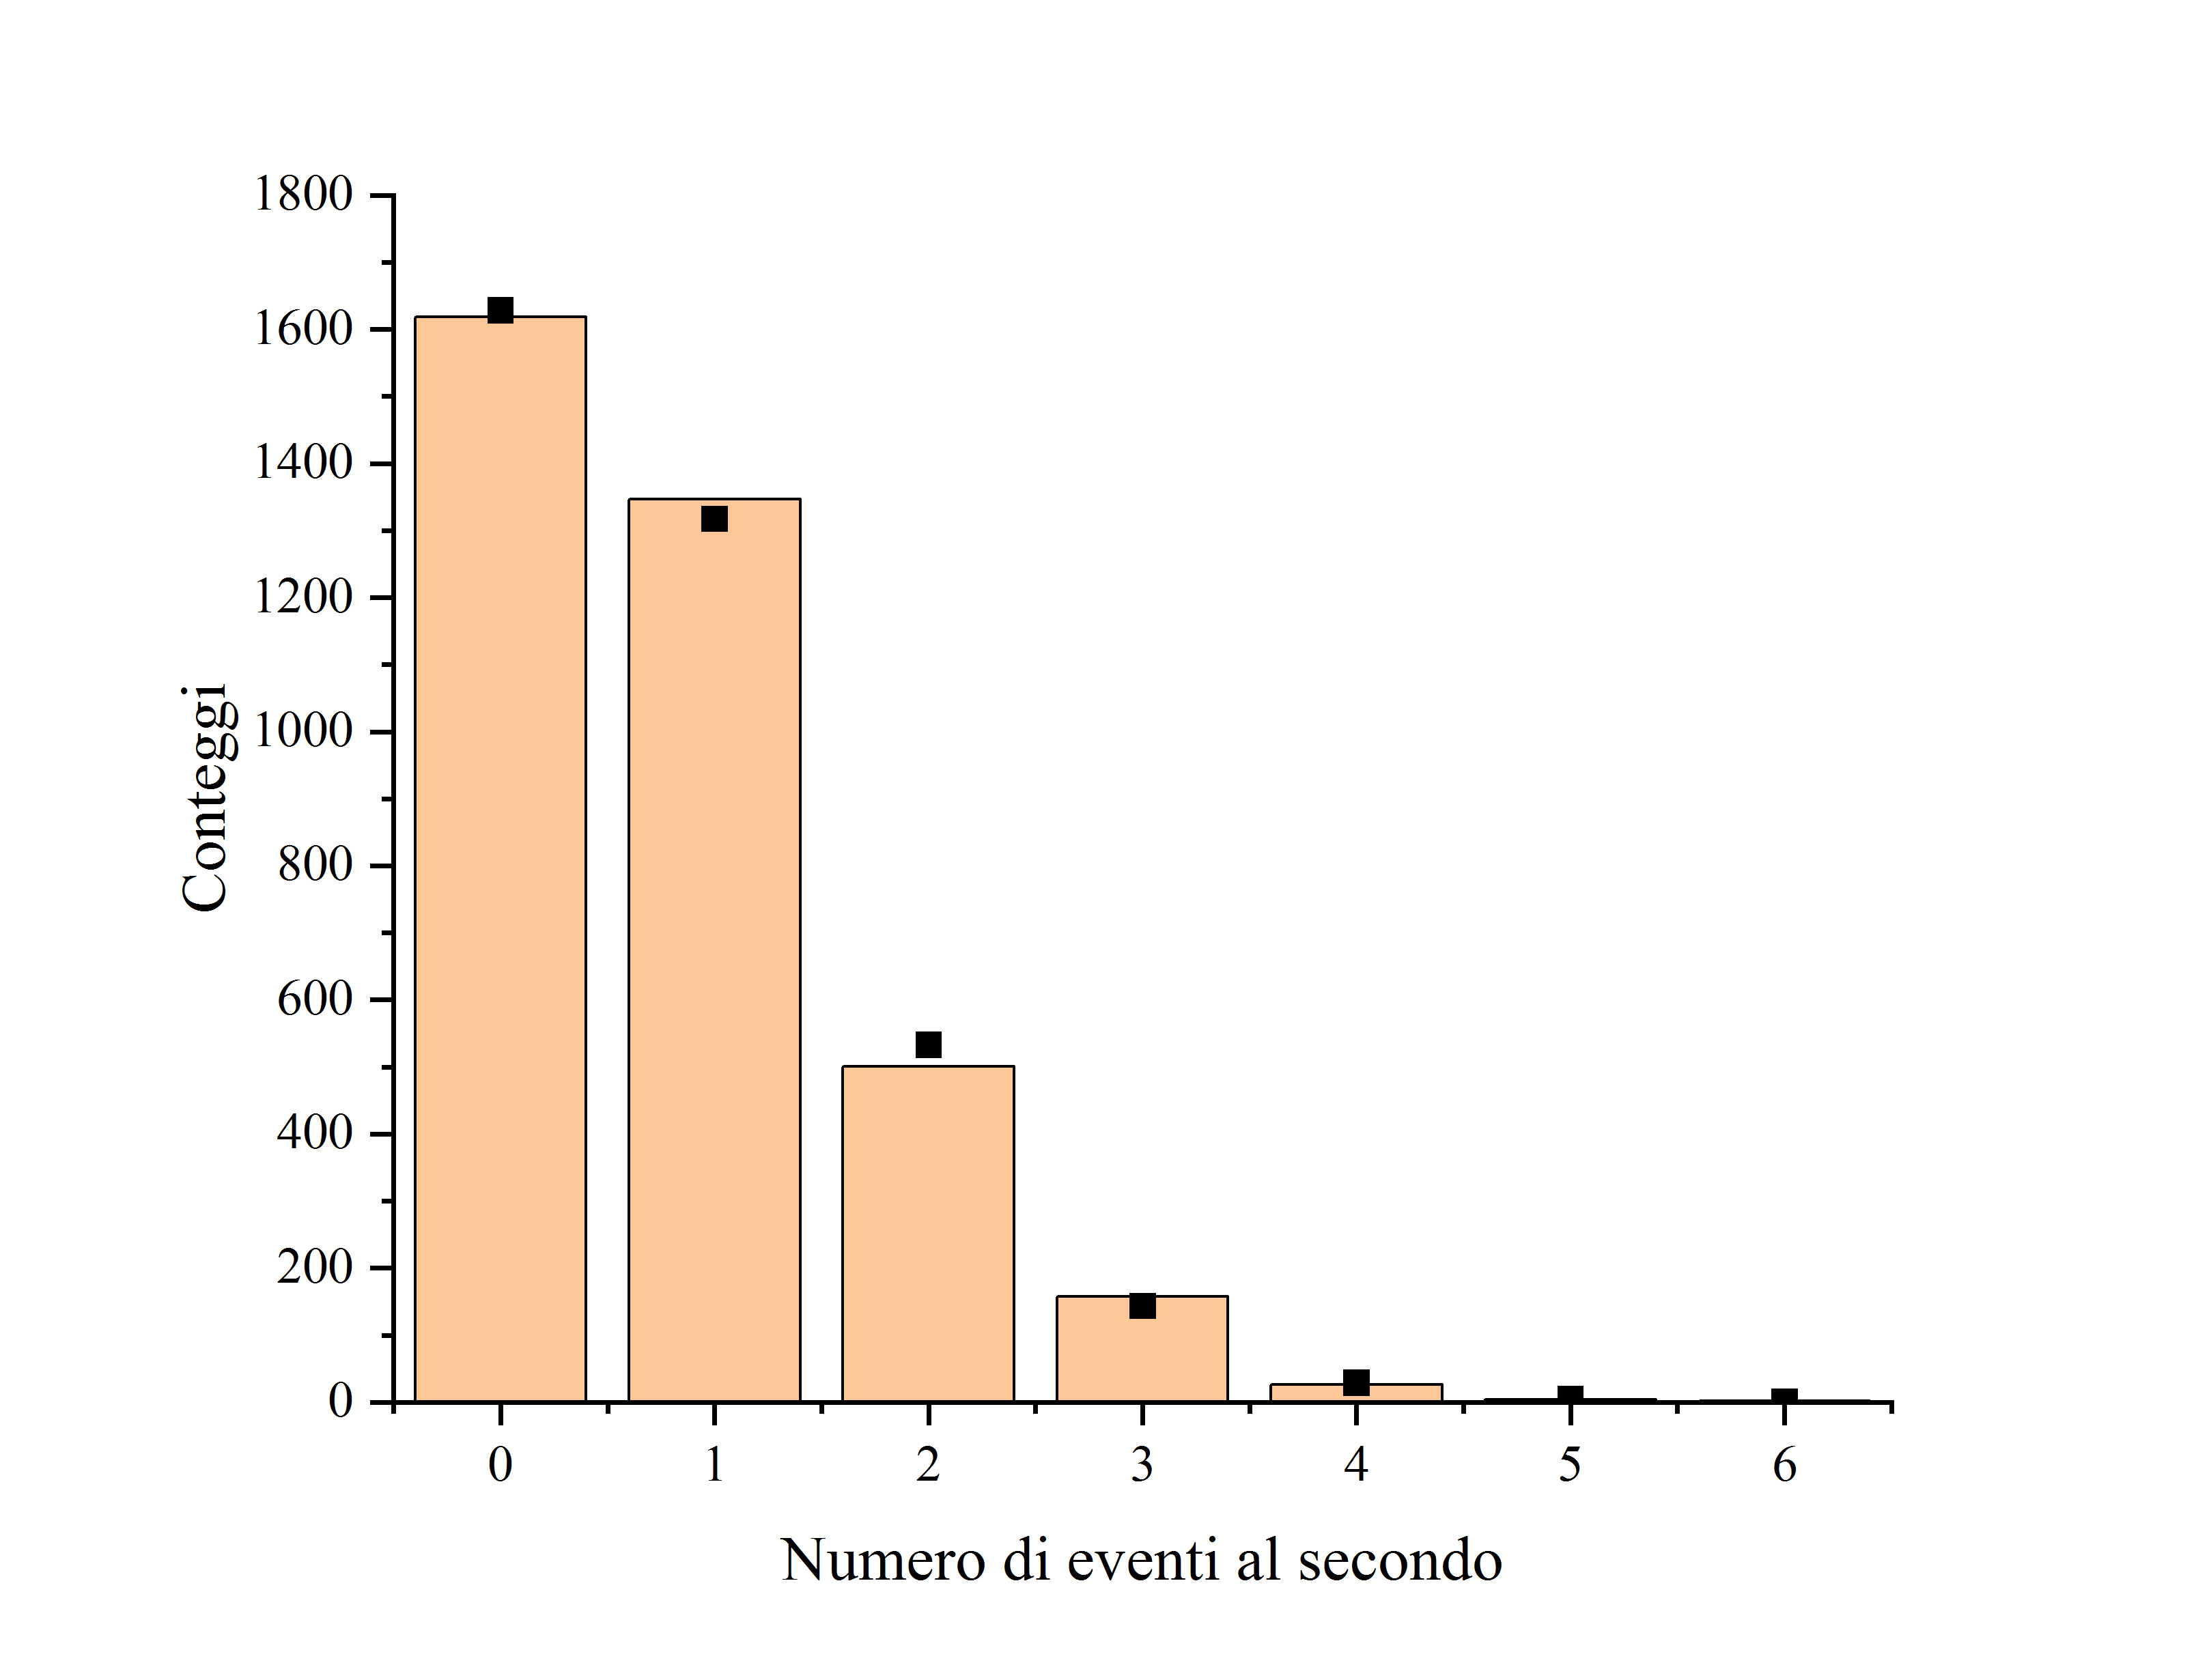
\includegraphics[trim={2cm .5cm 2.4cm 2.1cm},clip,width=.5\textwidth]{img/Geiger2.jpg}
        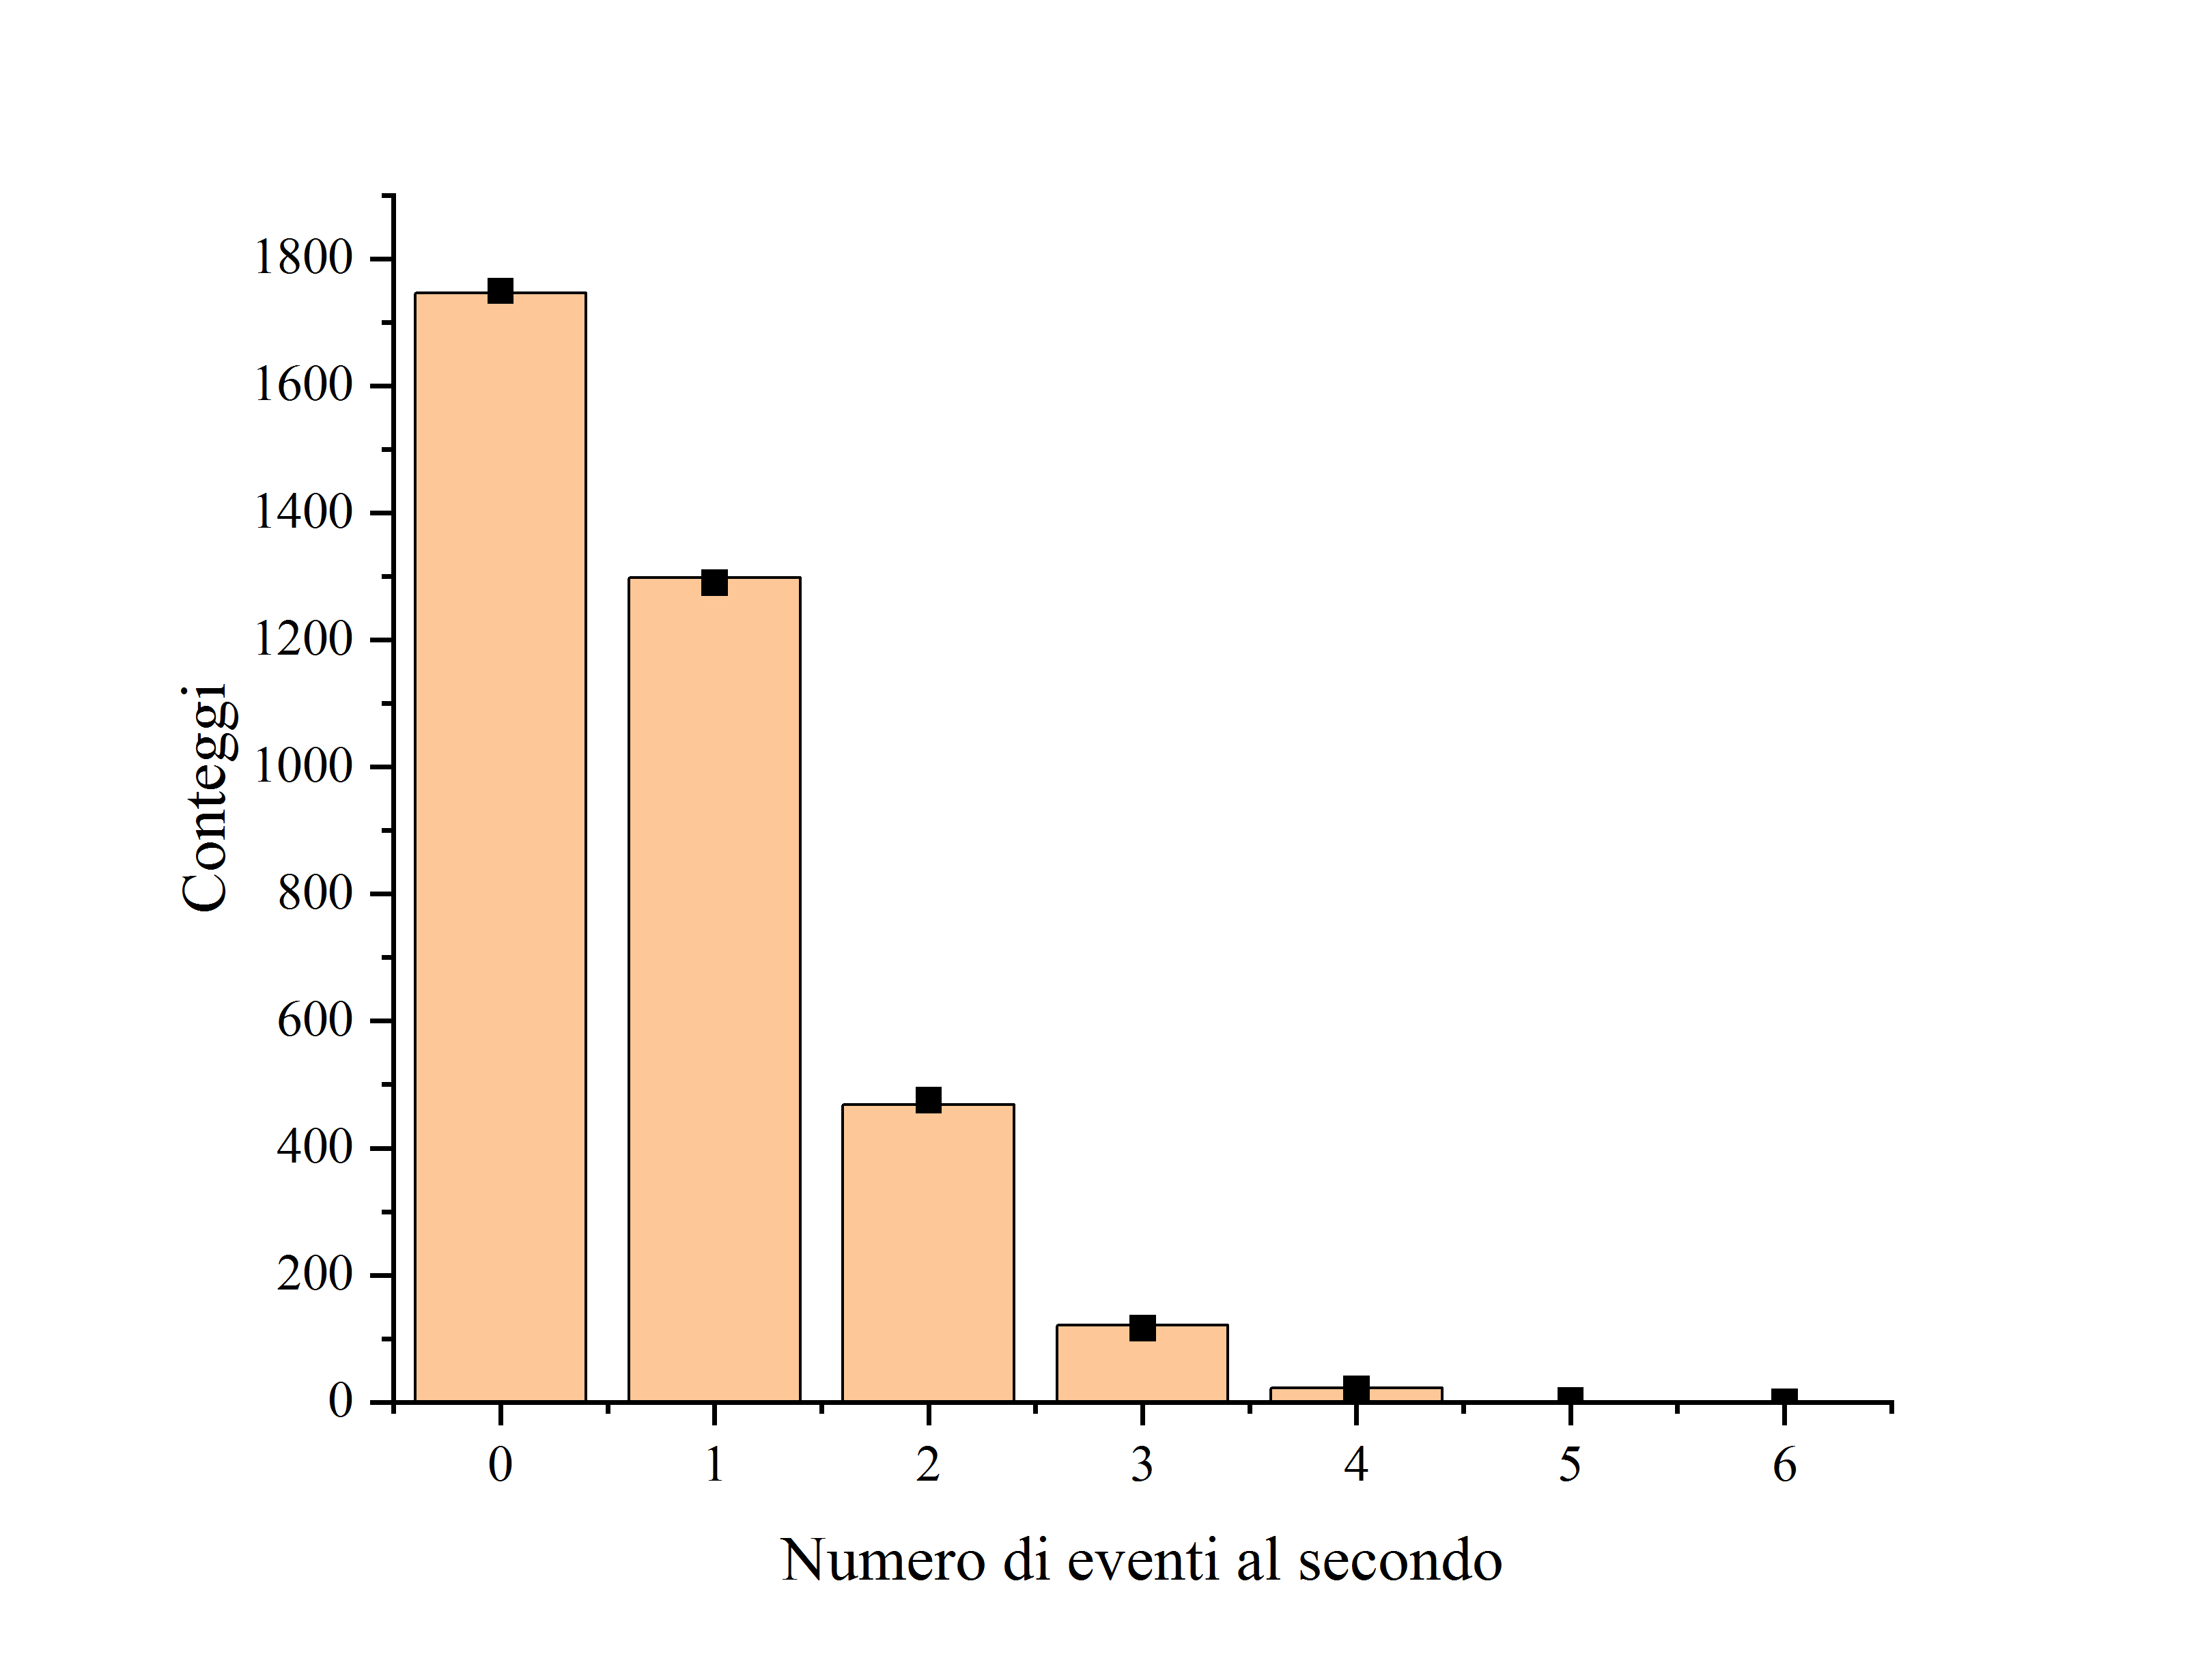
\includegraphics[trim={2cm .5cm 2.4cm 2.1cm},clip,width=.5\textwidth]{img/Geiger1.jpg}
        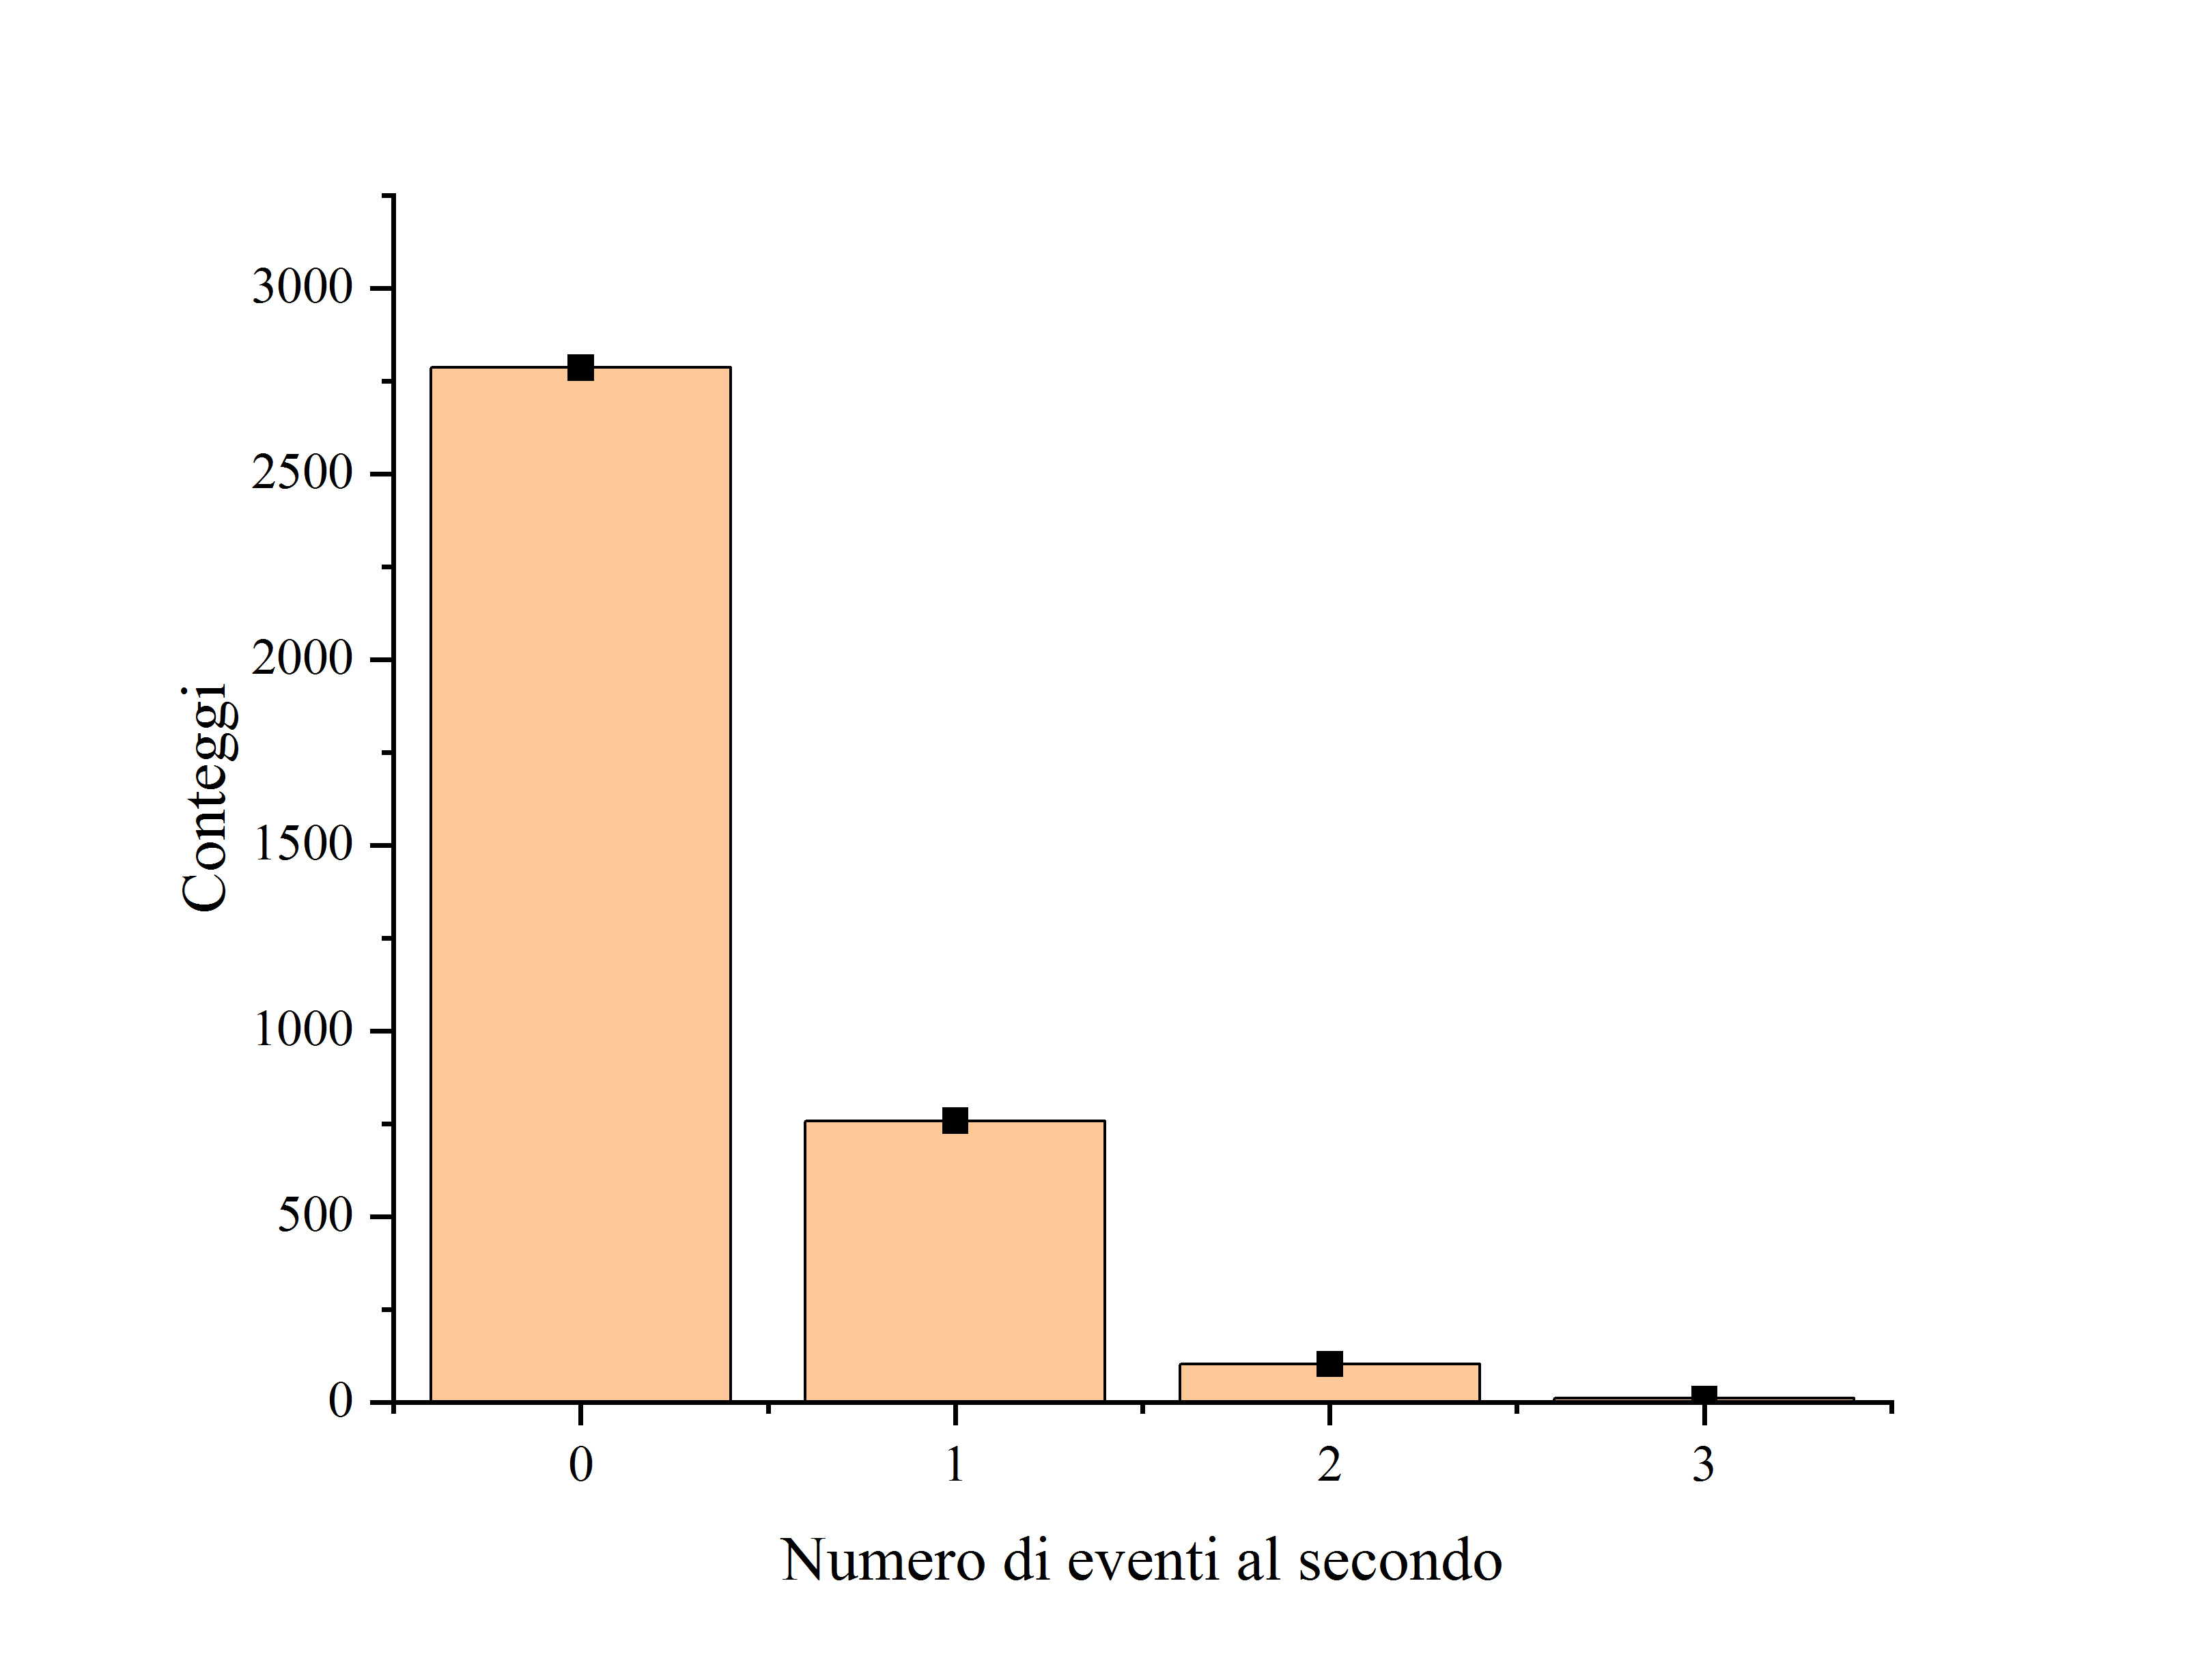
\includegraphics[trim={2cm .5cm 2.4cm 2.1cm},clip,width=.5\textwidth]{img/Geiger4.jpg}
        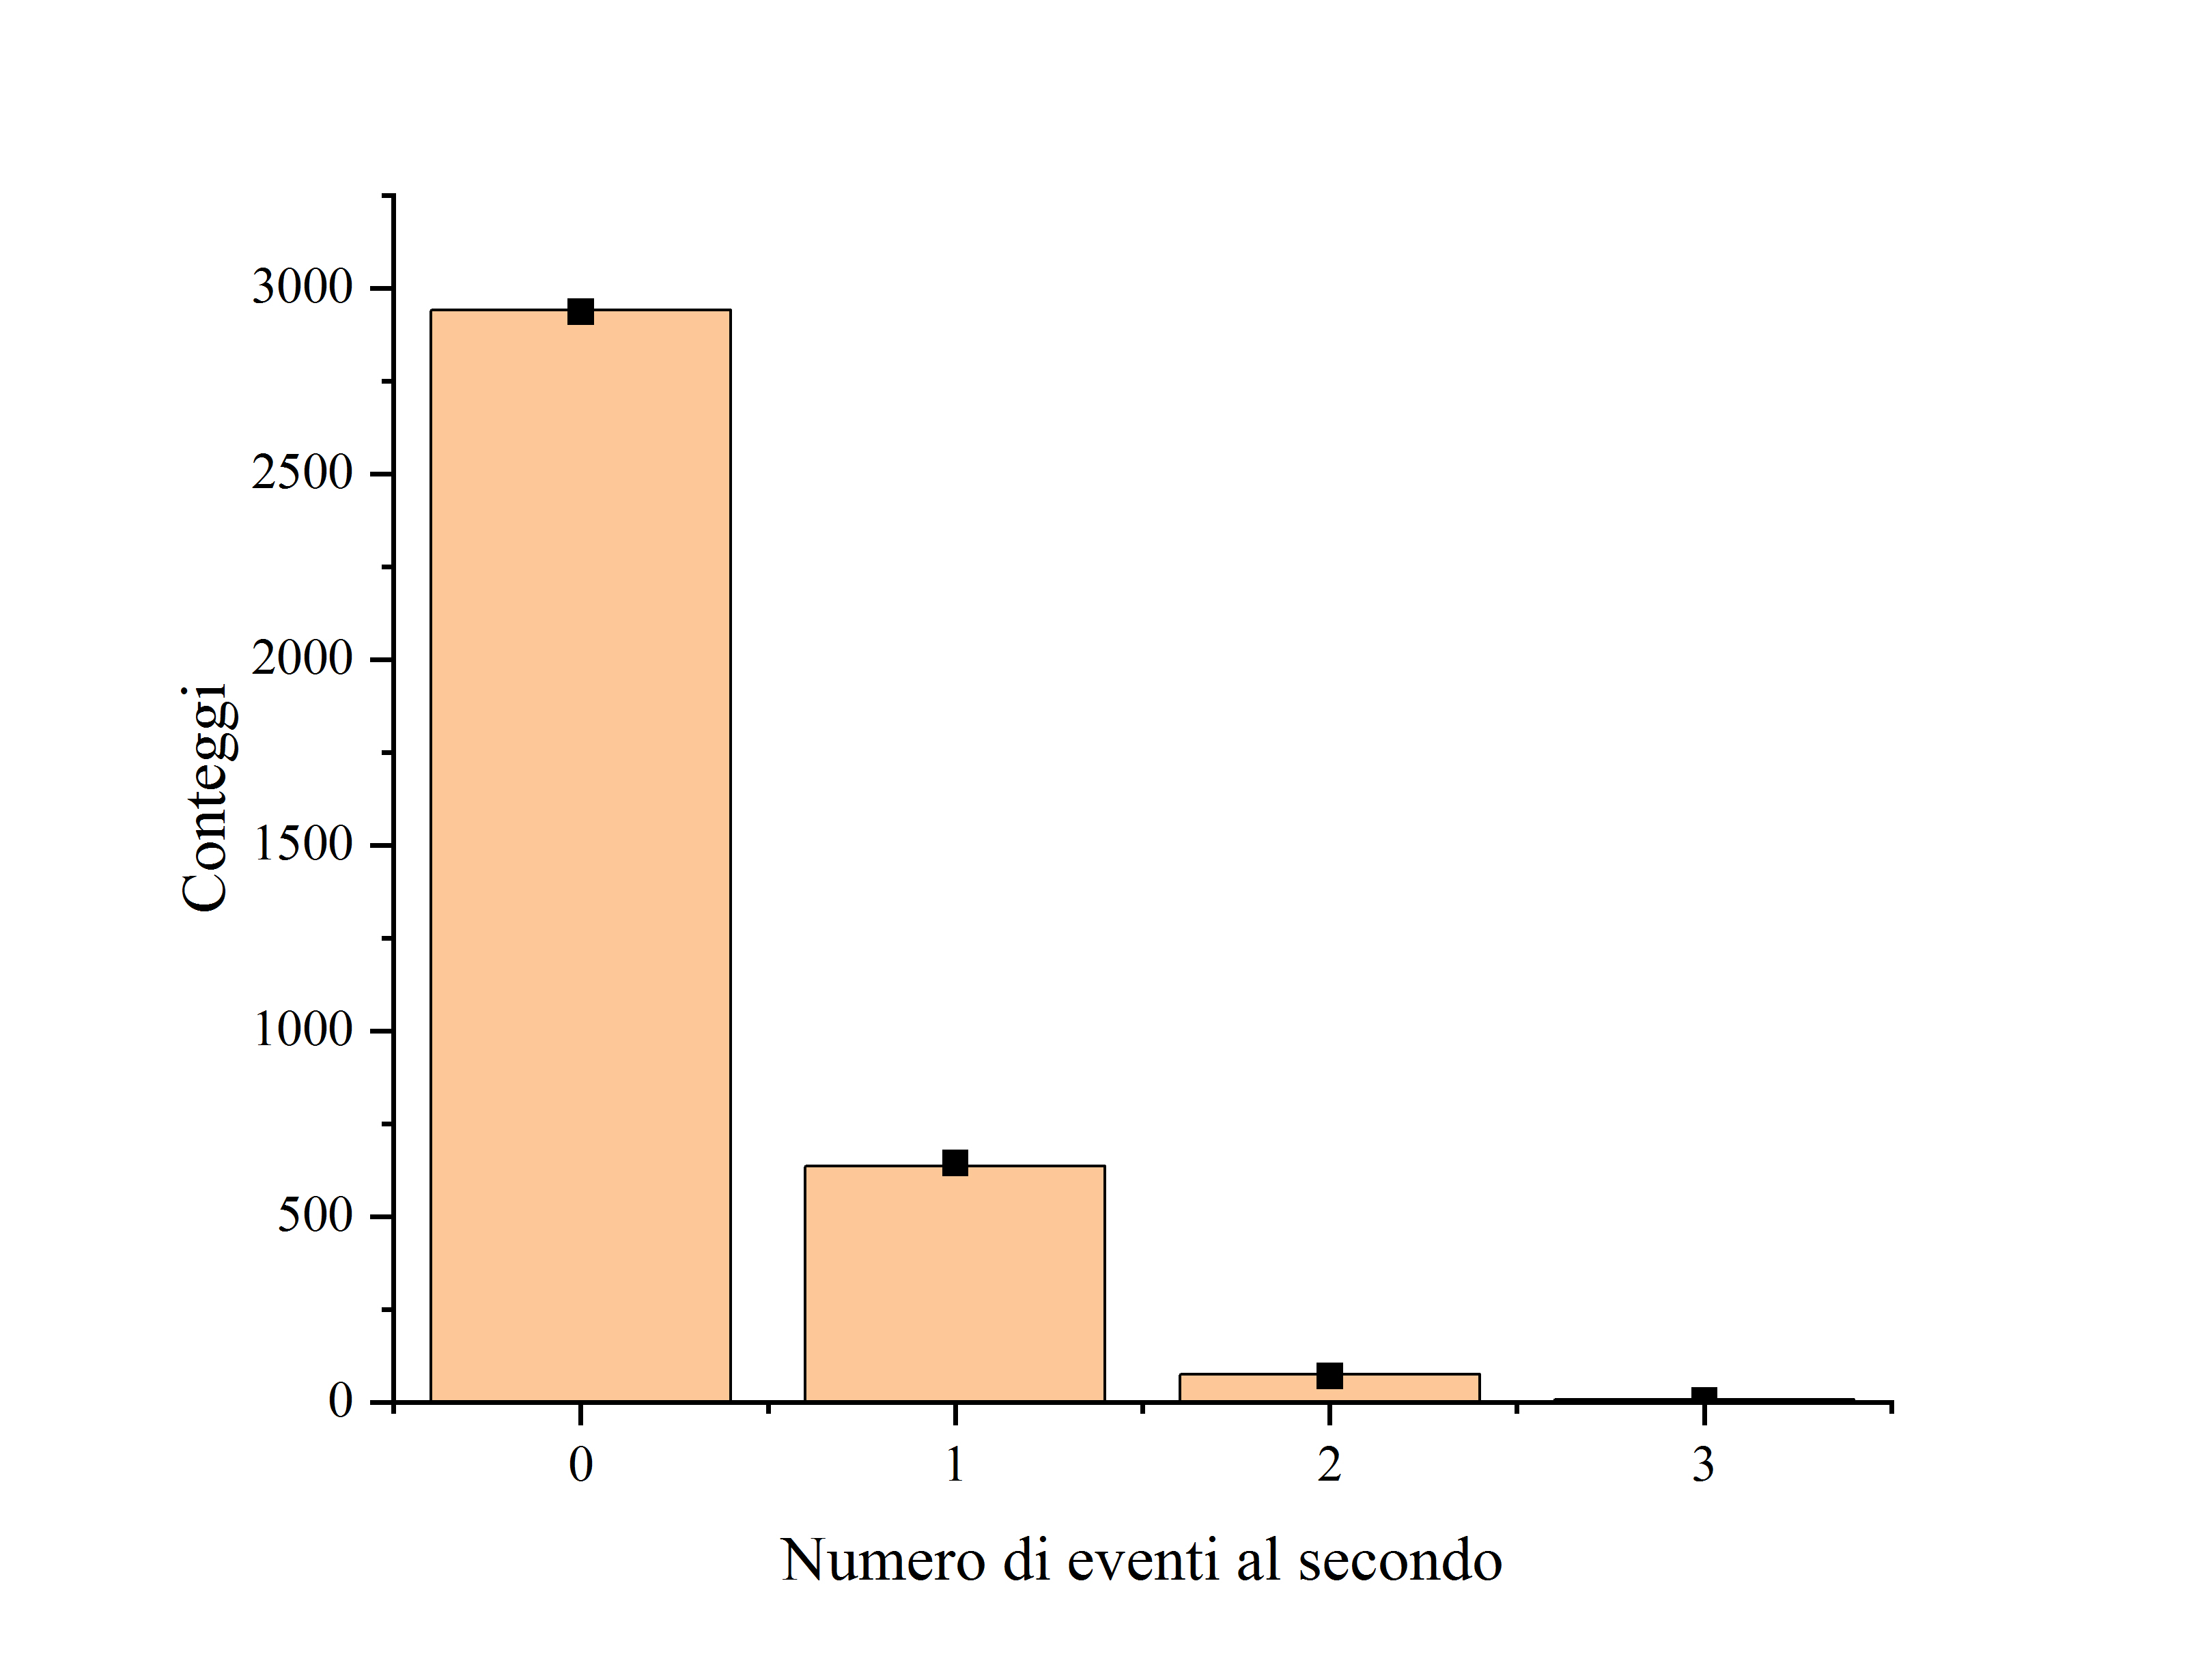
\includegraphics[trim={2cm .5cm 2.4cm 2.1cm},clip,width=.5\textwidth]{img/Geiger5.jpg}
    \end{figure}
\end{center}

Come si può osservare, le distribuzioni ottenute si allineano molto bene alle
distribuzioni di Poisson

\begin{center}
    \begin{tblr}{ |Q[c,m]|Q[c,m]|Q[c,m]|Q[c,m]| }
        \hline
        $i$ & $d_i\;\;(\unit{cm})$ & $d_i^{-2}\;\;(\unit{m^{-2}})$ & $\overline{\gamma_i}$ \\
        \hline
        1 & $9.5\pm0.1$  & $111\pm2$      & $0.809\pm0.015$\\
        2 & $10.3\pm0.1$ & $94.3\pm1.8$   & $0.737\pm0.014$\\
        3 & $26.5\pm0.1$ & $14.24\pm0.11$ & $0.272\pm0.009$\\
        4 & $41.2\pm0.1$ & $5.89\pm0.03$  & $0.219\pm0.008$\\
        \hline
    \end{tblr}
    \begin{figure}[H]
        % trim={< v > ^}
        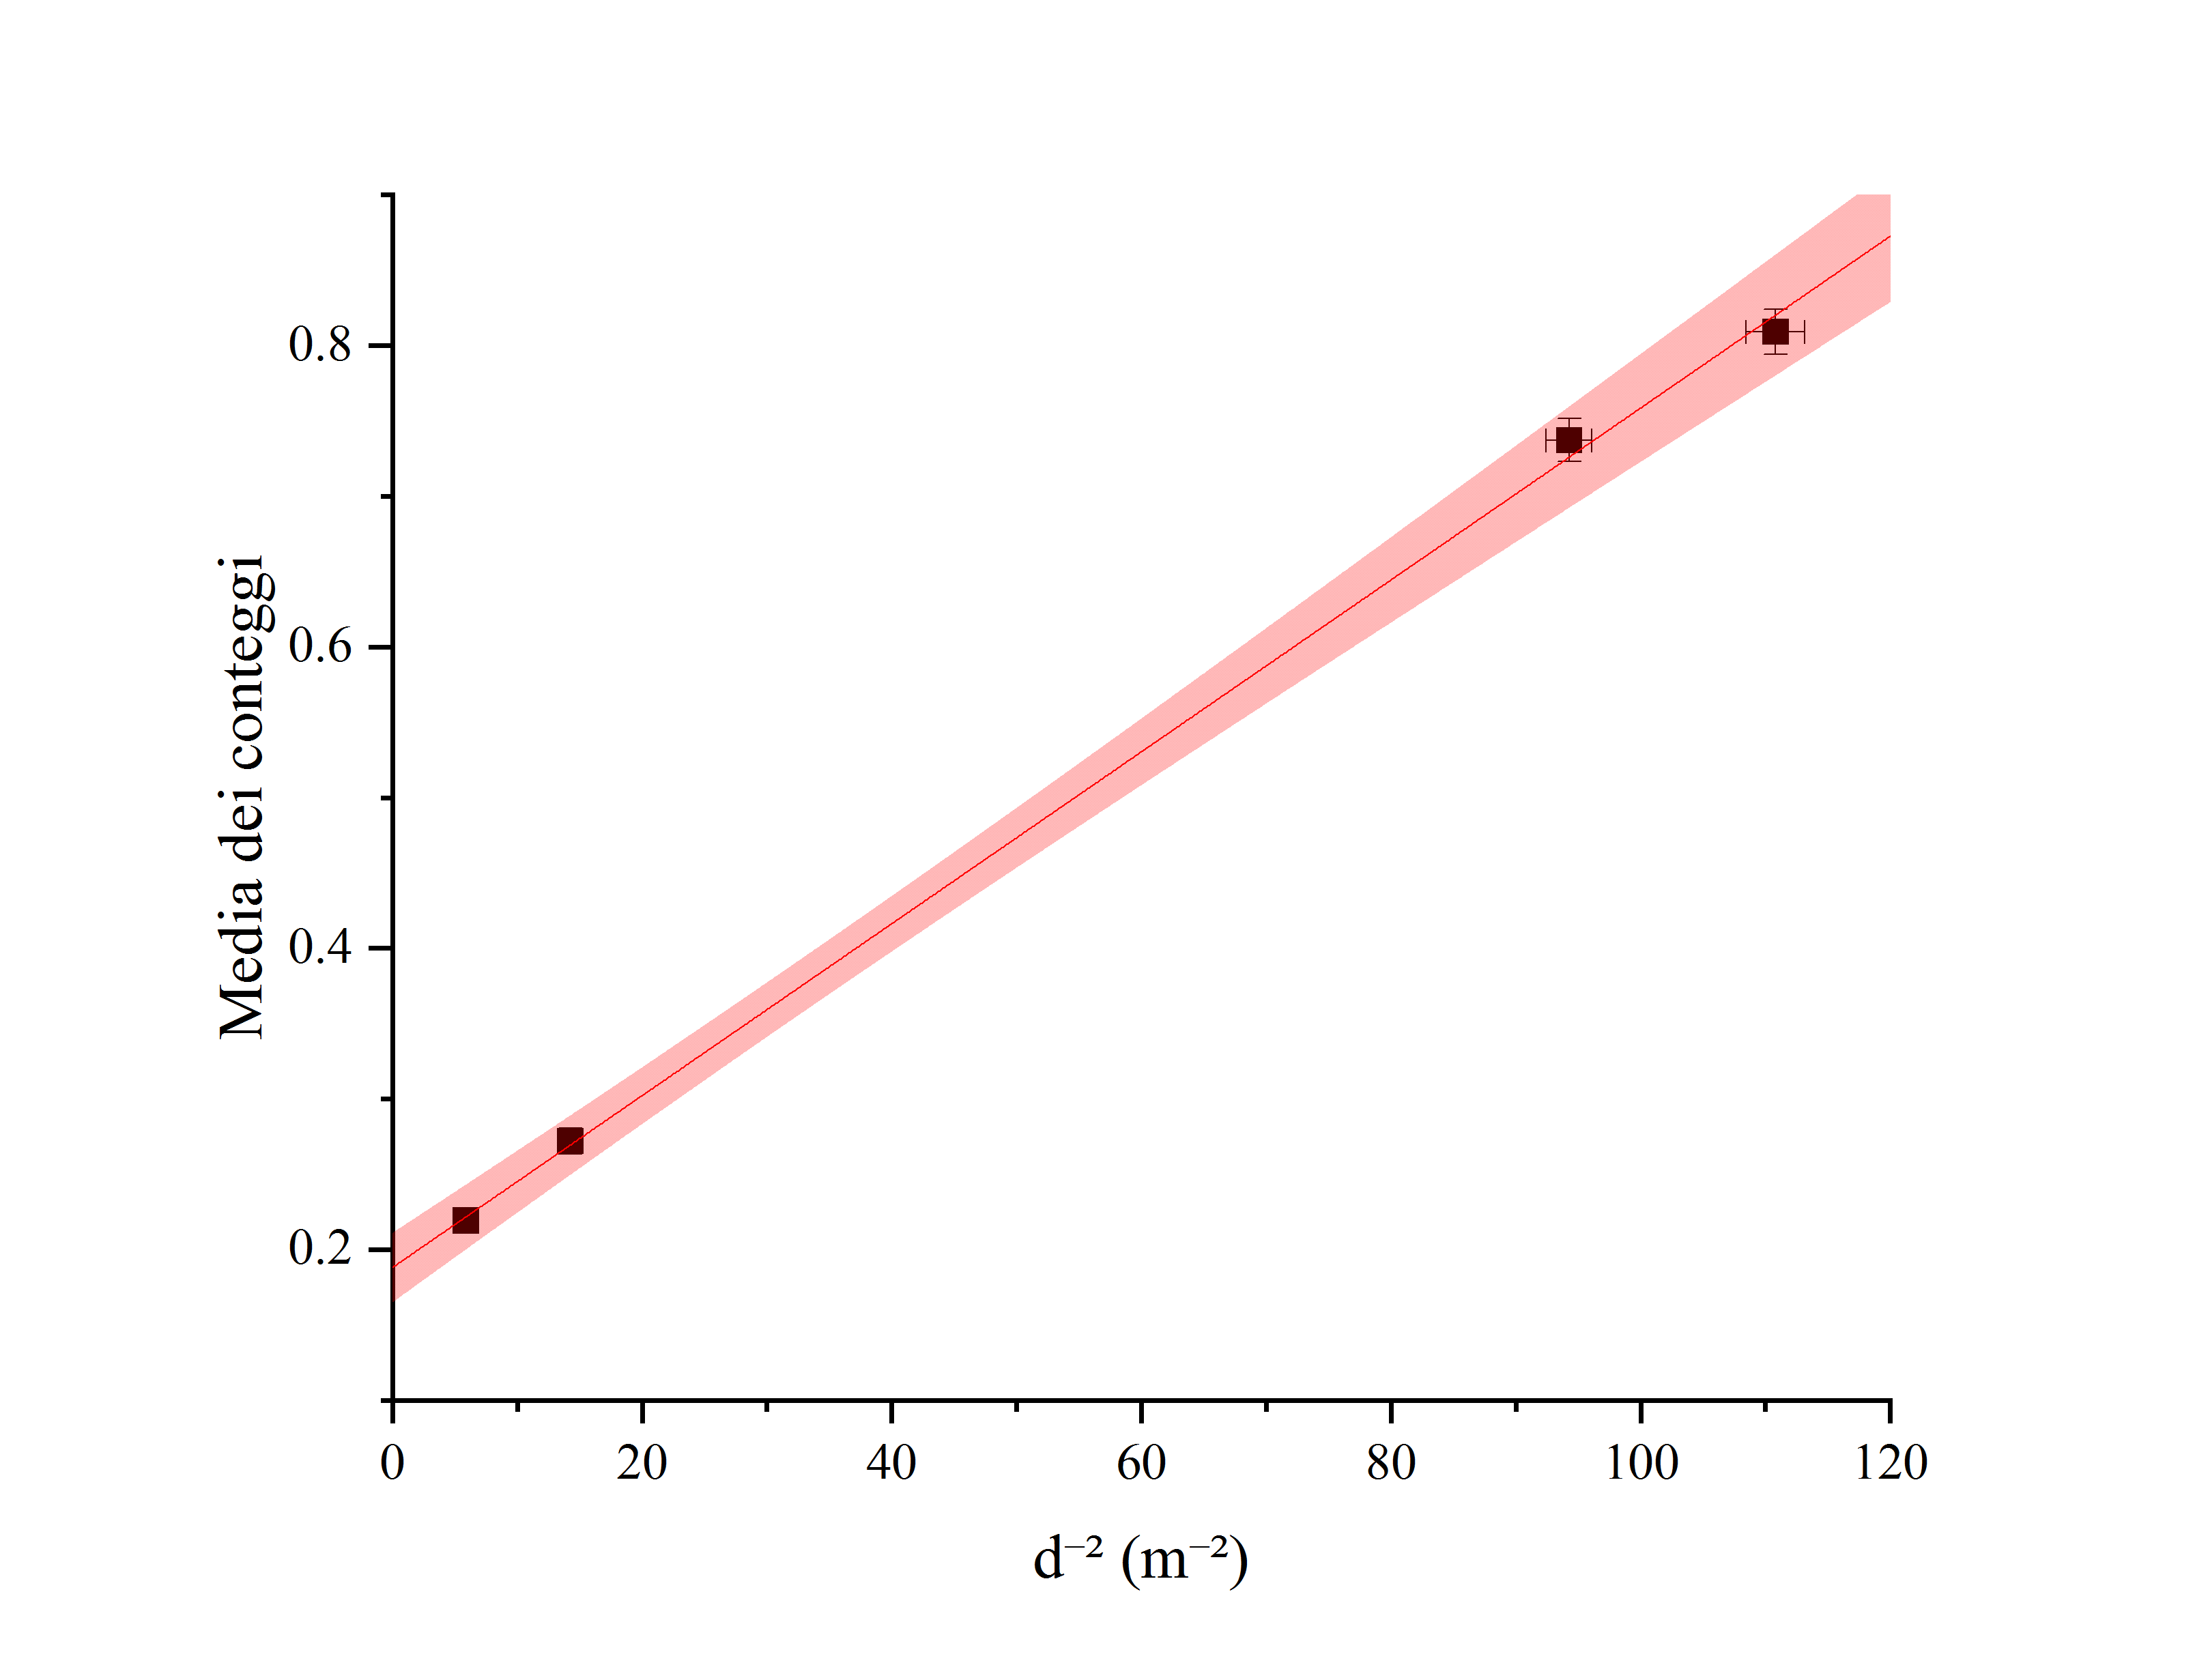
\includegraphics[trim={2cm .5cm 2cm 2.1cm},clip,width=\textwidth]{img/Regressione.png}
        \caption{
            La retta di regressione (in rosso) e la sua regione di incertezza (in rosa).
        }
    \end{figure}
\end{center}

\subsection{Conclusioni}
Per valutare numericamente la consistenza tra i due valori di $k$ ottenuti,
abbiamo calcolato il seguente valore (numero puro):
\[
    \varepsilon =
    \frac{
        \left|\left(k_\text{statica}\right)_\text{best} - \left(k_\text{dinamica}\right)_\text{best}\right|
    }{
        \delta k_\text{statica} + \delta k_\text{dinamica}
    }
\]
Allora $k_\text{statica}$ e $k_\text{dinamica}$ sono consistenti se e solo se $\varepsilon \le 1$.

Nel nostro caso, $\varepsilon = 1.33$. Il gruppo di lavoro ha ipotizzato che
questa inconsistenza (comunque contenuta, seppur non trascurabile) fra le due
misure possa essere ragionevolmente giustificata dalla difficoltà incontrata
nel ridurre al minimo le oscillazioni in direzione perpendicolare a $\vec{g}$;
considerato inoltre che la posizione dei fototraguardi non era ottimale, ciò
potrebbe avere ulteriormente influenzato la distribuzione dei tempi. È in
effetti possibile osservare che le distribuzioni da noi ottenute non sono,
il più delle volte, del tutto simmetriche: la moda sembra essersi spostata
leggermente a sinistra – un possibile sintomo dell'influenza di un
errore sistematico sulle misure.

\pagebreak
\begin{appendices}
    \section{Codice Rust per $\cdot10^{12}$ lanci di sei dadi}
    Qui riportiamo il codice Rust, da noi scritto, che ci ha permesso di
    lanciare virtualmente $6\cdot10^{12?}$ dadi in maniera estremamente
    efficiente.

    \inputminted[linenos, mathescape]{rust}{src/main.rs}
\end{appendices}

\end{document}
